%
% Niniejszy plik stanowi przykład formatowania pracy magisterskiej na
% Wydziale MIM UW.  Szkielet użytych poleceń można wykorzystywać do
% woli, np. formatujac wlasna prace.
%
% Zawartosc merytoryczna stanowi oryginalnosiagniecie
% naukowosciowe Marcina Wolinskiego.  Wszelkie prawa zastrzeżone.
%
% Copyright (c) 2001 by Marcin Woliński <M.Wolinski@gust.org.pl>
% Poprawki spowodowane zmianami przepisów - Marcin Szczuka, 1.10.2004
% Poprawki spowodowane zmianami przepisow i ujednolicenie 
% - Seweryn Karłowicz, 05.05.2006
% Dodanie wielu autorów i tłumaczenia na angielski - Kuba Pochrybniak, 29.11.2016

% dodaj opcję [licencjacka] dla pracy licencjackiej
% dodaj opcję [en] dla wersji angielskiej (mogą być obie: [licencjacka,en])
\documentclass[licencjacka]{style}


% Dane magistranta:
%\autor{Imię Nazwisko}{123456}


% Dane magistrantów:
\autor{Magdalena Grabowska}{372701}
\autori{Michał Kukuła}{371127}
\autorii{Klaudia Laks}{371151}
\autoriii{Przemysław Perkowski}{371308}
%\autoriv{Autor nr Cztery}{432145}
%\autorv{Autor nr Pięć}{342011}

\title{Miejsca Obsługi Podróżnych}


\tytulang{Parking places at rest areas on highways and expressways in Poland}

%kierunek: 
% - matematyka, informacyka, ...
% - Mathematics, Computer Science, ...
\kierunek{informatyka}

% informatyka - nie okreslamy zakresu (opcja zakomentowana)
% matematyka - zakres moze pozostac nieokreslony,
% a jesli ma byc okreslony dla pracy mgr,
% to przyjmuje jedna z wartosci:
% {metod matematycznych w finansach}
% {metod matematycznych w ubezpieczeniach}
% {matematyki stosowanej}
% {nauczania matematyki}
% Dla pracy licencjackiej mamy natomiast
% mozliwosc wpisania takiej wartosci zakresu:
% {Jednoczesnych Studiow Ekonomiczno--Matematycznych}

% \zakres{Tu wpisac, jesli trzeba, jedna z opcji podanych wyzej}

% Praca wykonana pod kierunkiem:
% (podać tytuł/stopień imię i nazwisko opiekuna
% Instytut
% ew. Wydział ew. Uczelnia (jeżeli nie MIM UW))
\opiekun{dr. hab. Aleksego Schuberta\\
  }

% miesiąc i~rok:
\date{Czerwiec 2018}

%Podać dziedzinę wg klasyfikacji Socrates-Erasmus:
\dziedzina{ 
%11.0 Matematyka, Informatyka:\\ 
%11.1 Matematyka\\ 
%11.2 Statystyka\\ 
11.3 Informatyka\\ 
%11.4 Sztuczna inteligencja\\ 
%11.5 Nauki aktuarialne\\
%11.9 Inne nauki matematyczne i informatyczne
}

%TODO Tu trzeba wpisać jakieś numerki ale nie umiem ich znaleźć.
%Klasyfikacja tematyczna wedlug AMS (matematyka) lub ACM (informatyka)
\klasyfikacja{D. Software \\ \\}


%TODO napisać jakieś
%Słowa kluczowe:
\keywords{symulacja, wizualizacja, Miejsce Obsługi Podróżnych, miejsce parkingowe, aplikacja okienkowa, aplikacja mobilna, strona internetowa, zajętość miejsc parkingowych, natężenie ruchu}

% Tu jest dobre miejsce na Twoje własne makra i~środowiska:
\newtheorem{defi}{Definicja}[section]

% koniec definicji

\usepackage{graphicx}
\usepackage[breaklinks=true]{hyperref}
\usepackage{dirtree}
\usepackage{graphicx,wrapfig,lipsum}
\usepackage{caption}
\usepackage[acronym,nonumberlist]{glossaries}

\renewcommand{\glossarysection}[2][]{}
\renewcommand{\glsgroupskip}{}

\makeglossaries

\newacronym{gddkia}{GDDKiA}{Generalna Dyrekcja Dróg Krajowych i Autostrad (nasz klient)}

\newacronym{mop}{MOP}{Miejsce Obsługi Podróżnych}

\newacronym{sdr}{SDR}{Średniodobowe natężenie ruchu}

\newacronym{gui}{GUI}{Graficzny interfejs użytkownika}

\newacronym{rn}{RN}{React Native}

\newacronym{api}{API}{Interfejs programowania aplikacji (ang. Application programming interface)}

\newacronym{zpp}{ZPP}{Zespołowy Projekt Programistyczny}

\newacronym{rid}{RID}{Rozwój Innowacji Drogowych}

\glsaddall

\begin{document}

\maketitle
\begin{abstract}
  W~pracy opisano implementację systemu dotyczącego Miejsc Obsługi Podróżnych
  przy autostradach i~drogach ekspresowych w Polsce. Podstawowe składowe tego
  systemu to aplikacje Mopnik i~Mopsim. Są one aplikacjami okienkowymi
  korzystającymi ze wspólnego interfejsu graficznego. Służą do~przeprowadzania
  krótko- i~długoterminowych predykcji ruchu na drogach oraz zajętości miejsc
  parkingowych na~Miejscach Obsługi Podróżnych. Pozostałe dwie części to
  aplikacja mobilna oraz strona internetowa przeznaczone dla kierowców
  poruszających się po drogach. Informują one o~zajętości miejsc parkingowych
  na każdym \acrshort{mop}-ie w danym momencie oraz predykcji ich zajętości w niedalekiej
  przyszłości.
\end{abstract}

\tableofcontents
%\listoffigures
%\listoftables


\chapter{Słowniczek}
\printglossaries

\chapter{Wprowadzenie}
\section{Rozwój sieci drogowej w Polsce}

Jeszcze pod koniec XX w. w Polsce znajdowało się zaledwie ok. 500km autostrad i~dróg ekspresowych. Pomimo licznych planów rozwojowych, które przyjmowane były w~okresie PRL i~pierwszych latach III RP, większość dróg budowana była z dużymi opóźnieniami, a niektórych odcinków nie realizowano wcale.\newline
Dopiero przyjęty pod koniec lat 90. program budowy sieci autostrad i dróg ekspresowych w~Polsce, mimo wielu modyfikacji jest na bieżąco realizowany. Jako przyczyny\cite{siec-drogowa-IIIrp} przyspieszenia budowy dróg szybkiego ruchu w Polsce wymienia się między innymi: duże zainteresowanie problemem, wzrost liczby pojazdów, dotacje z europejskiego Funduszu Spójności, a także dotacje Unii Europejskiej. Dodatkowym impulsem mobilizującym instytucje rządowe do przyspieszenia prac w tym kierunku stało się przyznanie organizacji Euro 2012 Polsce i Ukrainie.\newline
\begin{figure}[h]
\caption{Rozwój sieci dróg ekspresowych i autostrad w Polsce na początku XX w.}
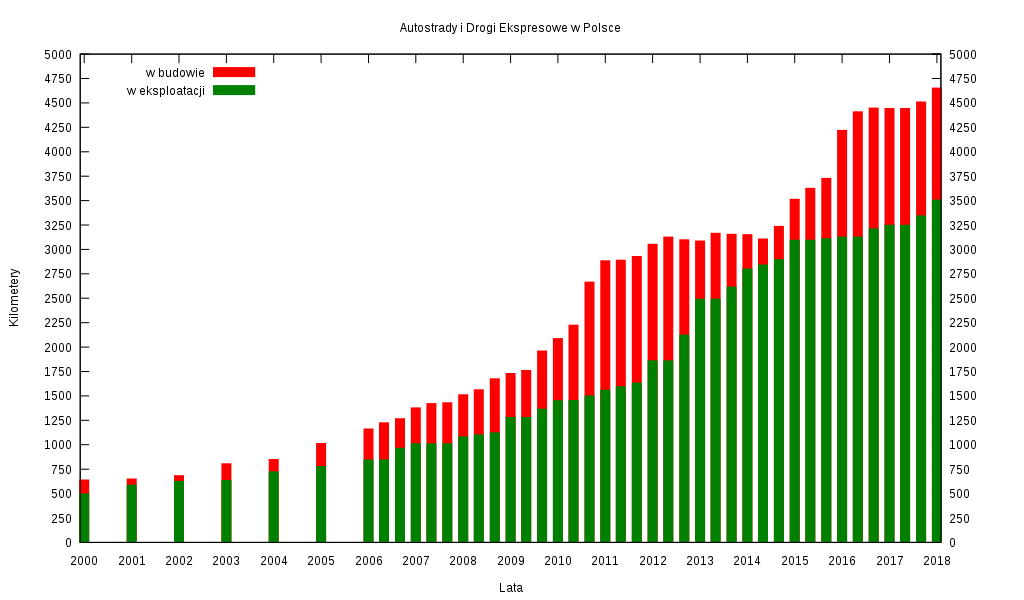
\includegraphics[width=\textwidth]{images/1024px-PL-Motorways.png}
\end{figure} \newline
Ostatnie lata to okres szczególnie intensywnego rozwoju sieci drogowej w Polsce. Budowa infrastruktury wiąże się również z potrzebą zapewnienia podróżnym bezpieczeństwa i komfortu.
\begin{figure}[h]
\caption{Sieć autostrad i dróg ekspresowych w Polsce (styczeń 2018r.). Na zielono -- odcinki zrealizowane, na czerwono -- odcinki w budowie, na szaro -- odcinki planowane.}
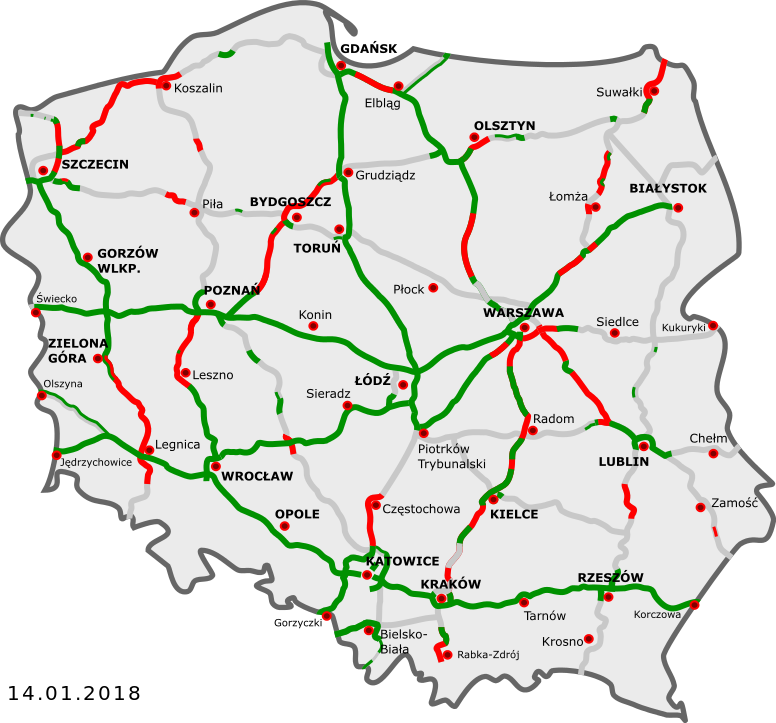
\includegraphics[width=\textwidth]{images/2018.png}
\end{figure}

\section{Miejsca Obsługi Podróżnych}
Miejsce Obsługi Podróżnych (\textbf{MOP}) to teren wydzielony w pasie drogowym (w bliskim sąsiedztwie drogi), wyposażony w parking oraz w infrastrukturę zapewniającą komfort i odpoczynek podróżnym\cite{gddkia-mop}. MOP-y powstają tylko przy autostradach i drogach ekspresowych.\newline
MOP-y w Polsce dzielimy na trzy kategorie:
\begin{enumerate}
    \item \textbf{MOP kategorii I} -- o funkcji wypoczynkowej, wyposażony w stanowiska postojowe (parking), jezdnie manewrowe, urządzenia wypoczynkowe, sanitarne i oświetlenie; dopuszcza się wyposażenie w obiekty małej gastronomii.
    \item \textbf{MOP kategorii II} -- o funkcji wypoczynkowo-usługowej, wyposażony w obiekty, o~których mowa w~punkcie 1. oraz w stację paliw, stanowiska obsługi pojazdów, obiekty gastronomiczno-handlowe, punkty informacji turystycznej.
    \item \textbf{MOP kategorii III} -- o funkcji wypoczynkowej i usługowej, wyposażony w~obiekty, o~których mowa w~punkcie 2., obiekty noclegowe oraz inne obiekty handlowo-usługowe w zależności od potrzeb.
\end{enumerate}
\begin{figure}[h]
\caption{Aktualne (styczeń 2018r.) pozycje MOP-ów w Polsce (na niebiesko). MOP-y planowane (na czerwono).}
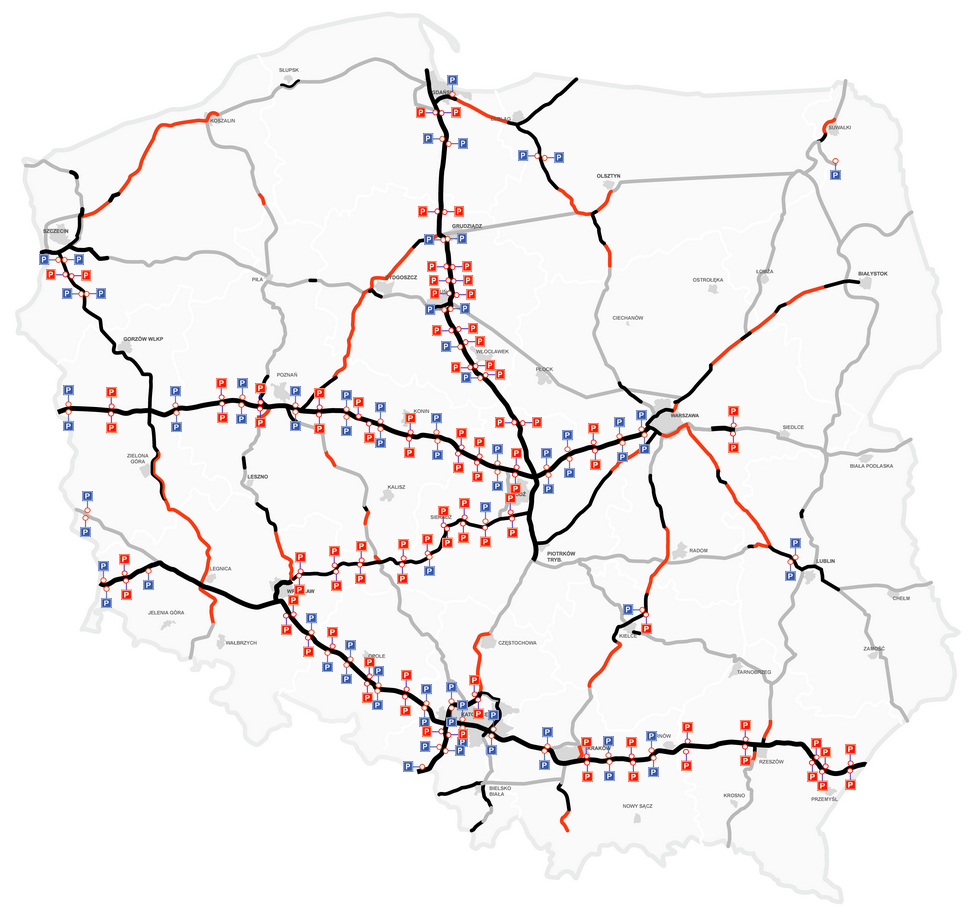
\includegraphics[width=\textwidth]{images/mopymap.png}
\end{figure}

\section{Problemy związane z budową MOP-ów}
Intensywny rozwój sieci drogowej, a co za tym idzie również szybki wzrost liczby MOP-ów w~Polsce, stwarza szereg problemów z nimi związanych:
\begin{enumerate}
    \item \textbf{Problemy administracyjno-prawne} -- \acrshort{gddkia} systematycznie prowadzi kolejne przetargi na~dzierżawę MOP zlokalizowanych zarówno przy autostradach jak i drogach ekspresowych. Dzierżawa nieruchomości MOP generuje przychody, które systematycznie zasilają budżet Krajowego Funduszu Drogowego. Nieatrakcyjne warunki umowy lub~lokalizacja punktu mogą zniechęcać potencjalnych najemców.
    \item \textbf{Lokalizacja MOP-ów} -- efektywne rozmieszczenie MOP-ów powinno uwzględniać takie parametry jak: odległość od najbliższych MOP-ów, natężenie odcinka drogi, odległość od węzłów komunikacyjnych.
    \item \textbf{Liczba miejsc parkingowych i ich układ} -- MOP-y powinny dysponować taką liczbą miejsc parkingowych, by zapewnić możliwość odpoczynku podróżującym także w warunkach wzmożonego ruchu. Rozmieszczenie miejsc parkingowych powinno zapewnić kierowcom komfort podczas poruszania się pojazdem na terenie punktu.
\end{enumerate}

\section{Symulacja ruchu drogowego w Polsce}
Efektywne rozmieszczenie coraz większej liczby MOP-ów jest jednym z głównych wyzwań stojących przed planistami dróg. Powinno ono uwzględniać wszystkie kwestie poruszone w~poprzednim rozdziale. Jednak rozwój sieci drogowej w Polsce na niespotykaną wcześniej skalę sprawia, że zadanie to jest coraz trudniejsze. Może się okazać, że dane dotyczące natężenia ruchu na danym odcinku drogi, odległości od najbliższych MOP-ów czy węzłów komunikacyjnych są niewystarczające i trudno na ich podstawie określić wykorzystanie MOP-a w okresach wzmożonego ruchu sezonowego lub w przyszłości, wraz z dalszym rozwojem infrastruktury drogowej. Przydatnymi danymi, wykorzystywanymi w modelowaniu ruchu drogowego, są macierze podróży, określające liczbę pojazdów poruszających się pomiędzy danymi parami punktów w zadanym okresie. Planista dróg, wyposażony w macierze podróży, chciałby na ich podstawie wiedzieć:
\begin{enumerate}
	\item Jakie jest natężenie ruchu na poszczególnych odcinkach drogi?
	\item Jak dodanie lub usunięcie (np. w wyniku tymczasowego zatrzymania ruchu) odcinka drogi wpłynie na to natężenie?
	\item Jaka część podróżnych, jadąca danym odcinkiem drogi, chciałaby skorzystać z MOP-a?
\end{enumerate}
Pomocny w przeprowadzeniu tej analizy może okazać się \textbf{Mopsim} -- program komputerowy symulujący ruch pojazdów na
sieci dróg krajowych i autostrad w Polsce.

\section{Przewidywanie liczby potrzebnych miejsc parkingowych}
Mając dane dotyczące natężenia ruchu na danym odcinku drogi (pochodzące z
przeprowadzonych pomiarów lub symulacji) można spróbować określić sumaryczną
liczbę miejsc parkingowych potrzebnych na tym odcinku. W tym celu powszechnie
wykorzystuje się różne metodyki, będące zwykle prostymi wzorami matematycznymi.

Przykład metodyki: 
$$ P_T = N_T \times SDR_T \times WS_T $$
gdzie:
\begin{itemize}
  \item $T$ -- typ pojazdu
  \item $P_T$ -- liczba potrzebnych miejsc parkingowych na 15km drogi
  \item $N_T$ -- wskaźnik przeliczeniowy uwzględniający np. typ MOP-u
  \item $SDR_T$ -- średni dobowy ruch w roku w analizowanym kierunku 
  \item $WS_T$ -- wskaźnik zmienności sezonowej
\end{itemize}
Program \textbf{Mopnik} będzie miał za zadanie umożliwienie korzystania z
takich metodyk -- ich kalibracji (ręcznego wprowadzania niektórych parametrów),
wczytywania potrzebnych danych (np. średniodobowego natężenia ruchu)
oraz obliczania liczby potrzebnych miejsc parkingowych. \\
Program będzie też umożliwiał integrację z systemem \textbf{Mopsim} dzięki
czemu możliwe będzie zastosowanie wyżej wymienionych metodyk do danych
pochodzących z symulacji, jeśli okaże się, że wyniki rzeczywistych pomiarów są
niepełne. 


\section{Zajętość MOP-ów i dostępne usługi}

Jednym ze wspomnianych wcześniej problemów związanych z budową MOP-ów jest dobór odpowiedniej liczby miejsc parkingowych. Dodatkowo, miejsca te należy odpowiednio podzielić pomiędzy różne typy pojazdów: samochody osobowe, samochody ciężarowe, autobusy, pojazdy przewożące substancje niebezpieczne itd. Podróżni mają też różne potrzeby związane z postojem -- od szybkiego zatankowania samochodu, przez obiad z rodziną na świeżym powietrzu, do spędzenia nocy w kabinie. \newline Aktualnie informację o znajdujących się na MOP-ie usługach można uzyskać ze znaków informacyjnych umieszczonych kilka kilometrów przed zjazdem. Jednak takie oznaczenia nie~odpowiadają na kilka ważnych pytań, które możemy mieć na dowolnym etapie podróży:
\begin{enumerate}
	\item Za ile kilometrów znajduje się najbliższa stacja benzynowa? 
	\item Czy starczy mi paliwa do następnej, ponieważ tutaj jest duża kolejka?
	\item Czy na tym MOP-ie jest monitoring?
	\item Czy na tym MOP-ie są wolne miejsca parkingowe? (ten problem jest ważniejszy z~punktu widzenia kierowców pojazdów wielkogabarytowych)
	\item Jaka będzie zajętość miejsc parkingowych za~godzinę?
\end{enumerate}

Odpowiedzią na te pytania będzie \textbf{Mopsik} (MOP -- System Informowania Kierowców) -- aplikacja mobilna i strona internetowa.


\section{Nasze zadanie}
W ramach zajęć \acrshort{zpp} postanowiliśmy podjąć się implementacji prototypów wyżej opisanych programów.
Badania są finansowane ze środków projektu pt. ,,Miejsca parkingowe na MOP'' finansowanego przez NCBiR/GDDKiA w ramach wspólnego przedsięwzięcia ,,RID'', umowa DZP/RID-I-44/8/NCBR/2016.
\chapter{Mopnik}\label{r:Mopnik}

\section{Przypadki użycia}
Inżynier \acrshort{gddkia} może:
\begin{enumerate}
  \item Wprowadzać dane dotyczące \acrshort{sdr} oraz położenie MOP-ów z pliku.
  \item Wyświetlić wprowadzone dane na mapie.
  \item Wybrać metodykę, ustawić jej parametry i na jej podstawie wyznaczyć
    liczbę potrzebnych miejsc parkingowych na odcinku drogi oraz na konkretnym
    MOP-ie.
  \item Wyświetlić wyniki na mapie.
  \item Edytować sieć drogową. 
  \item Wyświetlić wyniki symulacji przeprowadzonych za pomocą systemu
    \textbf{Mopsim} dotyczących:
    \begin{enumerate}
      \item Długo- i krótkoterminowych predykcji \acrshort{sdr}.
      \item Krótkoterminowej predykcji zajętości MOP-ów.
    \end{enumerate}
  \item Zapisać wyniki przeprowadzanych analiz do pliku.
\end{enumerate}

\section{Architektura}
\textbf{Mopnik} jest napisany w języku Java z użyciem narzędzia Apache
Maven automatyzującego budowę programu.
\subsubsection{Wykorzystywanie biblioteki}
Implementacja opiera się na wykorzystaniu następujących bibliotek dla języka
Java:
\begin{itemize}
\item Swing -- biblioteka graficzna służąca do stworzenia \acrshort{gui} aplikacji.
\item JXMapViewer2 -- biblioteka zapewniająca swingowy JPanel renderujący
  kafelki mapy (\url{https://github.com/msteiger/jxmapviewer2}).
\item osm-parser -- biblioteka parsująca pliki .osm do obiektów w Javie
  (\url{https://github.com/imintel/osm-parser}).
\item opencsv -- biblioteka do parsowania plików CSV
  (\url{http://opencsv.sourceforge.net/})
\end{itemize}
Oprócz zewnętrznych bibliotek, program korzysta też z będącej częścią tego
projektu biblioteki \textbf{Mopsim}. 
\subsubsection{Dane wejściowe}
Użytkownik programu ma możliwość wprowadzenia danych dotyczących \acrshort{sdr}
oraz położenia MOP-ów z pliku w formacie CSV. Pliki te muszą spełniać pewne
założenia (dotyczące formatu i kolejności pól) opisane w okienku służącym do
wczytywania pliku. Ponadto użytkownik ma możliwość wczytania sieci drogowej w
formacie OSM. Parsowaniem obu rodzajów plików zajmują się odpowiednie
biblioteki wymienione w poprzedniej sekcji.
\subsubsection{Wyświetlanie mapy}
\paragraph{} 
Mapa Polski, która jest wyświetlana po otwarciu programu, pochodzi z
serwisu \mbox{OpenStreetMap}. Kafelki są ściągane i renderowane według potrzeby, czyli
przy każdym przesunięciu czy przybliżeniu mapy. Takie rozwiązanie sprawia, że
użytkownik musi być przez cały czas korzystania z programu podłączony
do internetu. Jest możliwość stworzenia lokalnego serwera, hostującego
kafelki
\footnote{\url{https://switch2osm.org/manually-building-a-tile-server-16-04-2-lts/}}, a
następnie zmiany w kodzie adresu serwera na \textit{localhost}. Ze względu na
powszechny dostęp do internetu zrezygnowaliśmy z tego rozwiązania, ale warto
wiedzieć, że ono istnieje. 
\paragraph{}
Wczytywanie plików OSM daje następujące możliwości:
\begin{enumerate}
  \item Nanoszenie własnych oznaczeń na mapę -- na przykład kolorowanie
    konkretnych dróg.
  \item Modyfikowanie sieci drogowej. W tym wypadku zmiany nie zostaną
    wyświetlone tak jak istniejące drogi, ponieważ kafelki pochodzą z innego
    źródła. Wymagałoby to renderowania map w czasie działania programu, co
    spowolniłoby jego działanie. Zamiast tego, nowe drogi wizualizowane są
    za pomocą prostych odcinków łączących punkty wyznaczone przez użytkownika. 
    Możliwe jest jednak wprowadzanie własnych oznaczeń na dodanych
    odcinkach, tak jak na istniejących. 
\end{enumerate}

\section{Dokumentacja użytkowa i opis implementacji}

\chapter{Mopsim}\label{r:Mopsim}

\section{Przypadki użycia}
Inżynier \acrshort{gddkia} może:
\begin{enumerate}
  \item Wprowadzać dane dotyczące sieci drogowej z pliku osm.
  \item Wprowadzać dane dotyczące MOP-ów i macierze podróży z plików CSV.
  \item Edytować sieć drogową i dodawać lub usuwać MOP-y.
  \item Przeprowadzać symulację ruchu drogowego.
  \item Wyznaczać przewidywane natężenie ruchu na danym odcinku drogi.
  \item Wyznaczać przewidywaną zajętość MOP-ów i liczbę potrzebnych miejsc parkingowych.
  \item Generować raporty.
  \item Wyświetlić wyniki symulacji za pomocą \acrshort{gui} programu \textbf{Mopnik}.
\end{enumerate}

\section{Architektura}

\subsubsection{Modele mikro-, makroskopowe}
Modelem obliczeniowym w informatyce nazywamy model matematyczny, wykorzystujący zasoby komputerowe do zbadania zachowania złożonego systemu za pomocą symulacji\cite{model}. Modele obliczeniowe są obecnie wykorzystywane w bardzo wielu dziedzinach, m.in. do prognozy pogody, badania zmian klimatycznych, symulacji ruchu planet, a także w biologii czy medycynie. Jednym ze sposobów klasyfikacji modeli jest podział na modele mikro- i makroskopowe\cite{micmac}:
\begin{itemize}
\item w modelu mikroskopowym każda jednostka jest opisywana przez jej charakterystyczne atrybuty i zachowania
\item w modelu makroskopowym analizuje się zagregowane cechy grupy jednostek i ich oddziaływanie na cały system
\end{itemize}
\subsubsection{Model obliczeniowy oparty na agentach}
Jednym z intensywnie stosowanych i rozwijanych modeli obliczeniowych jest model oparty na~agentach (ang. \textit{agent-based model}).
Polega on na symulowaniu zachowań i oddziaływania między sobą zbioru autonomicznych agentów, w celu badania ich wpływ na cały system\cite{agent-based}. Zwykle agentom przyporządkowuje się uproszczone zachowania, a następnie umieszcza w pewnym miejscu i czasie. Następnie symuluje się podejmowane przez nich działania i oddziaływania między sobą w celu odtworzenia lub próby wyjaśnienia bardziej złożonych zjawisk. Modele obliczeniowe oparte na agentach stosuje się m.in. w biologii, ekologii czy naukach społecznych.
\subsubsection{System wieloagentowy}
    Nieco innym, choć pokrewnym pojeciem jest system wieloagentowy (ang. \textit{multi-agent system}). Jest to system komputerowy, złożony z wielu oddziałujących między sobą we wspólnym środowisku inteligentnych agentów. W odróżnieniu od modelu opartego na agentach, którego celem jest badanie złożonych procesów na podstawie zachowań poszczególnych jednostek, system wieloagentowy jest koncepcją programistyczną, w której agenci są wykorzystywani do rozwiązywania określonych problemów praktycznych lub inżynieryjnych. Systemy wieloagentowe często stosowane są w sytuacjach, gdy trzeba rozwiązać problemy o charakterze rozproszonym lub złożonych obliczeniowo, np. wyszukiwanie informacji w sieci, zarządzanie sieciami telekomunikacyjnymi, symulacja rynku, wspomaganie zarządzania w przedsiębiorstwie i kontrola ruchu lotniczego\cite{wiki-agent}. Poniższy schemat pokazuje ogólną zasadę działania systemu wieloagentowego. Każdy z agentów działa w środowisku, oddziałując na innych agentów i przeprowadzając obserwacje. Na ich podstawie, agent podejmuje decyzję o ewentualnej modyfikacji planu działania. Następnie agent ponownie wkracza do środowiska.
    \begin{figure}[h]
        \caption{Schemat działania systemu wieloagentowego}
        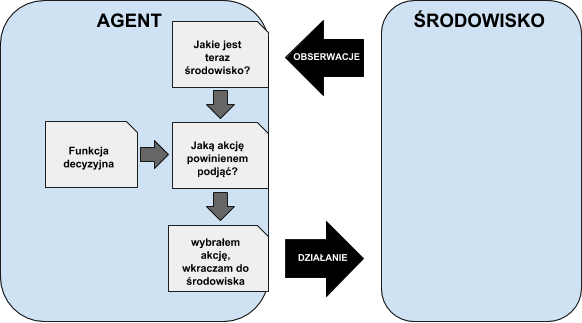
\includegraphics[width=\textwidth]{images/multi-agent.png}
    \end{figure}
\subsubsection{MATSim -- symulator ruchu drogowego}
MATSim (\textit{Multi-Agent Transport Simulation}) to open-sourcowy, rozszerzalny framework napisany w Javie służący do przeprowadzania symulacji ruchu drogowego. Jego głównymi założeniami jest mikroskopowe modelowanie ruchu oraz oparte na agentach symulowanie dziennych planów poszczególnych jednostek\cite{matsim}. MATSim został zaprojektowany, by modelować aktywności podczas pojedynczego dnia. MATSim oparty jest o zasadę koewolucyjności. Każdy z agentów, reprezentujących pojedynczych uczestników ruchu drogowego, optymalizuje swój codzienny plan, rywalizując z innymi agentami w różnych aspektach korzystania z infrastruktury drogowej.\\
Projekt MATSim został zapoczątkowany w 2004r. na Politechnice Federalnej w Zurychu. Od~tego czasu jest intensywnie rozwijany m.in. na tej uczelni, na Uniwersytecie Technicznym w~Berlinie, a także przez dziesiątki innych osób reprezentujących różne gałęzie nauki. MATSim został wykorzystany do przeprowadzenia symulacji ruchu drogowego m.in. w~Berlinie, Poznaniu, Seulu, Tel Avivie, Singapurze czy też dla całych Niemiec. Podejmowane były też próby wykorzystania go w celu modelowania ruchu lotniczego, symulowania ewakuacji czy~badania emisji spalin.
    \begin{figure}[h]
        \caption{Logo MATSim}
        
\includegraphics[width=\textwidth]{images/matsim_logo.png}
    \end{figure}
\subsubsection{MATSim -- pętla programu}
Działanie programu polega na przeprowadzeniu określonej liczby iteracji, reprezentowanych przez pętlę na poniższym schemacie. MATSim zaczyna swoje działanie, wczytując ustawienia konfiguracyjne dotyczące sieci drogowej, populacji agentów wraz z ich dziennymi planami oraz metadane o symulacji. Podczas iteracji, każdy z agentów optymalizuje swój początkowy plan. Każdy z nich posiada zdefiniowany zbiór planów, składających się z dziennego łańcucha aktywności i~wyniku punktowego, który może być interpretowany jako użyteczność w pojęciu ekonometrycznym. Przed każdą iteracją, agenci wybierają plan ze~swojego zbioru. Wybór ten zależy od wyników poszczególnych planów, które są obliczane po każdej pojedynczej symulacji. Pod koniec iteracji, część agentów (najczęściej ok. 10\%) może zmodyfikować wybrany przez siebie plan i dodać go do swojego zbioru planów. 
    \begin{figure}[h]
        \caption{Schemat działania MATSim}
        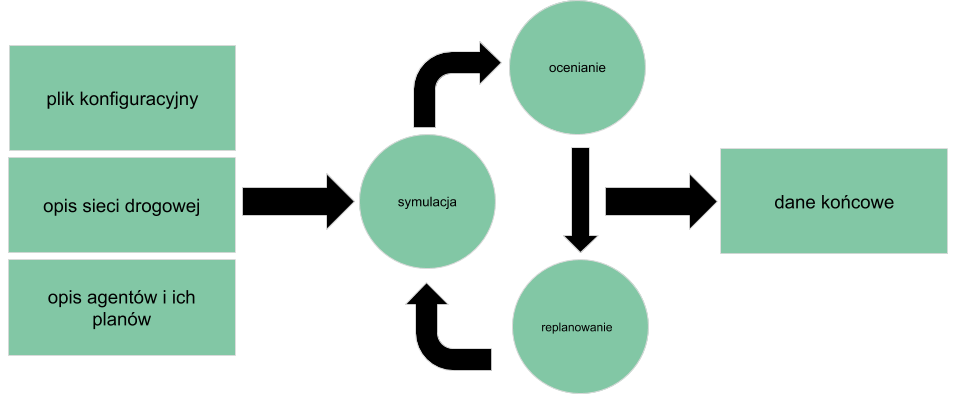
\includegraphics[width=\textwidth]{images/matsim-workflow.png}
    \end{figure}
\newpage
\subsubsection{Dlaczego MATSim?}
Przeprowadzone próby pokazały, że MATSim może być dobrym narzędziem do symulowania ruchu na drogach w Polsce, w celu zbadania zajętości MOP-ów. Co istotne, wstępne symulacje pokazały, że już jedna iteracja działania głównej pętli programu jest wystarczająca -- wynik jest bardzo zbliżony do optymalnego. Jest to zgodne z~intuicją -- w ruchu krajowym należy oczekiwać, że najkrótsza droga spośród dróg danego typu jest najbardziej optymalną, a~tworzące się korki nie są tak częste i~regularne, jak w intensywnym ruchu miejskim. Czynniki, które nas przekonały do wyboru frameworku MATSim to między innymi:
\begin{itemize}
\item licencja open-source
\item możliwość łatwego rozszerzenia o dodatkowe funkcjonalności, wiele gotowych przykładów
\item obszerna dokumentacja i dostęp do kodu źródłowego
\item możliwość zrównoleglania
\end{itemize}

\subsubsection{Mopsim -- schemat działania programu}
    \begin{figure}[h]
        \caption{Schemat działania programu Mopsim}
        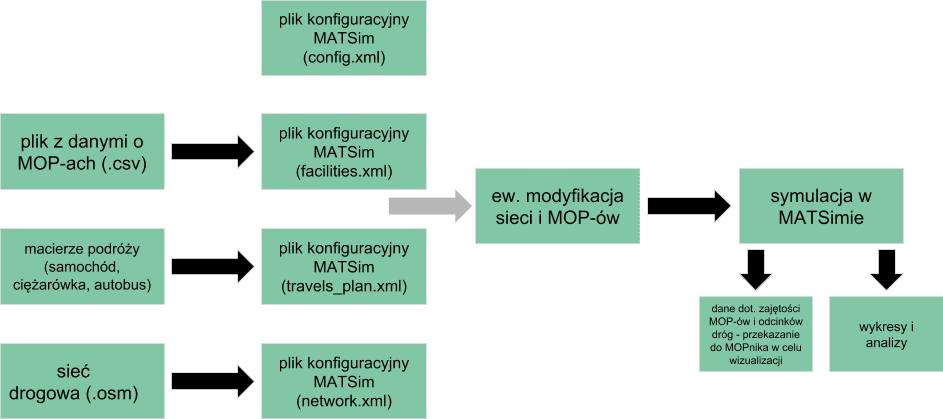
\includegraphics[width=\textwidth]{images/mopsim-workflow.png}
    \end{figure}
Program Mopsim wykorzystuje silnik programu MATSim do przeprowadzania symulacji. Poniższy schemat pokazuje zarys jego działania. Użytkownik programu Mopsim wprowadza dane wejściowe -- plik z danymi o MOP-ach w formacie csv, macierze podróży pomiędzy poszczególnymi miastami powiatowymi dla trzech rodzajów pojazdów -- samochodów osobowych, ciężarowych i autobusów w formacie csv oraz mapę sieci drogowej w formacie osm (\textit{OpenStreetMap}). Dane te są przetwarzane kolejno na odpowiednie pliki konfiguracyjne wykorzystywane przez MATSim -- opis obiektów powiązanych z odcinkami drogi (\textit{facilities}), opis agentów i ich planów oraz opis sieci drogowej. Użytkownik może dodatkowo zmodyfikować sieć dróg lub siatkę MOP-ów, dodając lub usuwając odpowiednie obiekty. Następnie przeprowadzana jest symulacja, w wyniku której tworzone są wykresy i inne dane analityczne, część których może być przekazana do programu Mopnik w celu wizualizacji.
\newpage
\subsubsection{Mopsim -- technologie}
W programie Mopsim wykorzystano następujące technologie:
\begin{itemize}
\item MATSim -- opisany wyżej
\item Java -- choć MATSim umożliwia też pisanie rozszerzeń w innym języku, zdecydowaliśmy się na wykorzystanie Javy jako języka programowania z uwagi na jej największą integrację z MATSimem. Dodatkowym atutem było nasze doświadczenie z pracy w tym języku, także w aspekcie programowania współbieżnego.
\item OpenStreetMap -- Mopsim korzysta z map OpenStreetMap do opisu sieci drogowej. Jest to projekt społeczności internetowej mający na celu stworzenie darmowej, swobodnie dostępnej mapy całej kuli ziemskiej. Jej atutem są gotowe rozwiązania umożliwiające edycję oraz integracja z MATSimem, który posiada moduł umożliwiający konwersję na~format używany do opisu dróg w symulacji.
\end{itemize}

\section{Dokumentacja użytkowa i opis implementacji}

\chapter{Mopsik -- Strona serwerowa - \acrshort{api}}\label{r:apka} 

Jednymi z podstawowych danych wczytywanych przez pisane przez nas programy (Mopsik--Mobile oraz Mopsik--Web) są dane o MOP-ach. Dane te są przedstawiane przez \acrshort{gddkia} w postaci ogólnie dostępnego skoroszytu programu Excel (rozszerzenie .xlsx) zamieszczanego na~stronie internetowej.
Predykcja zajętości MOP-ów odbywa się na podstawie różnych danych historycznych -- ankiet przeprowadzanych na MOP-ach oraz danych zbieranych za pomocą kamer.
Sensownym wydał się pomysł zbudowania wspólnego interfejsu do przekazywania tych danych naszym aplikacjom. W tym momenie z danych z API korzysta aplikacja mobilna MOPsik, strona internetowa oraz w programie Mopnik istnieje opcja pobrania danych z serwera.

Podczas tworzenia aplikacji pewnym problemem stało się posługiwanie różnymi układami współrzędnych przez różne komponenty, z~których korzystamy. Na~przykład dane na temat MOP-ów przez GDDKiA są w \href{https://pl.wikipedia.org/wiki/Uk\%C5\%82ad_wsp\%C3\%B3\%C5\%82rz\%C4\%99dnych_1992}{układzie 92}, Google Maps, którego używamy w naszej aplikacji mobilnej przyjmuje danych w układzie \href{https://pl.wikipedia.org/wiki/System_odniesienia_WGS_84}{WSG84}. Postanowiliśmy dodać do naszego API konwerter pomiędzy tymi układami.
\section{Przypadki użycia}
Serwer ze stroną internetową, klient aplikacji mobilnej oraz program Mopnik może:
\begin{enumerate}
\item Pobrać informacje na temat pozycji oraz dostępnych usprawnień na MOP-ach na podstawie najnowszego stanu przedstawionego do tej pory na stronie GDDKiA.
\item Pobrać dane o bieżącej zajętości MOP-ów.
\item Przekonwertować współrzędne pomiędzy układami WSG84 i układem 1992.
\end{enumerate}
\section{Architektura}
Na implementację API serwera składają się dwie części:
\begin{enumerate}
\item Skrypt cron
\item Aplikacja Django
\end{enumerate}
\paragraph{Cron}\mbox{}\\
Na serwerze zostało umieszczone polecenie, które regularnie sprawdza, czy na stronie GDDKiA nie pojawił się nowy arkusz .xlsx z MOP-ami. Jeśli tak, to jest wywoływana zdefiniowana przez nas w Django komenda $\textit{update\_mops\_db}$, która aktualizuje bazę danych.
\paragraph{Aplikacja Django}\mbox{}\\
Implementacja oparta jest o wersję 2.0 frameworku Django, Python 3.5 oraz bibliotekę django REST framework. Dane są przechowywane w bazie SQLite3. Na ten moment API odpowiada na następujące zapytania:
\begin{itemize}
\item /mops - zwraca wszystkie dane o MOP-ach agregowane w bazie danych
\item /taken - zwraca dane o zajętości MOP-ów agregowane w bazie danych
\item /wsg_to_92 - dla danej listy współrzędnych w formacie WSG84 zwraca listę współrzędnych w formacie 1992
\item /92_to_wsg - dla danej listy współrzędnych w formacie 1992 zwraca listę współrzędnych w formacie WSG84
\end{itemize}

\section{Dokumentacja użytkowa i opis implementacji}

\chapter{Mopsik -- Aplikacja mobilna}

\section{Przypadki użycia}
Zarówno w aplikacji mobilnej, jak i na stronie internetowej podróżny może:
\begin{enumerate}
\item Znaleźć MOP-a w wyszukiwarce lub na mapie.
\item Poznać procentową zajętość miejsc parkingowych na MOP-ie dla każdego z trzech typów pojazdów (samochód osobowy, samochód ciężarowy, autobus).
\item Poznać liczbę wolnych miejsc parkingowych oraz ich liczbę ogółem.
\item Znaleźć kontakt do operatora MOP-a.
\item Sprawdzić jakie usługi znajdują się na MOP-ie.
\item Wyświetlić wizualizację danych o zajętośći miejsc parkingowych.
\item Edytować preferencje wyświetlania danych dla konretnych typów pojazdów.
\end{enumerate}
Dodatkowo, w aplikacji mobilnej:
\begin{enumerate}
\item Mapa wyświetla aktualną lokalizację użytkownika, co umożliwia wybranie najbliższego MOP-a. 
\item Istnieje możliwość dodanie MOP-a do ulubionych i późniejsze wybranie go z~listy zapisanych.
\end{enumerate}


\section{Architektura i opis implementacji}

\subsection{Technologia}
\begin{figure}[!htb]
    \centering
    \begin{minipage}{.6\textwidth}
Aplikacja mobilna została napisana w języku \textbf{JavaScript} z użyciem biblioteki \textbf{React~Native} (dalej: RN). Dzięki temu pisząc jeden kod, otrzymujemy aplikację zarówno na telefony z Androidem, jak i iOS.
    \end{minipage}%
    \begin{minipage}{.4\textwidth}
        \centering
        
\includegraphics[width=5cm]{images/ReactNative.png}\label{RN_logo}
    \end{minipage}
\end{figure}

Aplikacja w \acrshort{rn} zbudowana jest z komponentów, które posiadają stan (obiekt słownikowy) inicjowany w konstruktorze. Funkcja \textit{render()} wywoływana jest przy pierwszym ładowaniu komponentu oraz przy każdej zmianie jego stanu. 

Z komponentów budujemy widoki, czyli wszystko co jest widoczne na ekranie w danym momencie.

Cała aplikacja objęta jest nawigatorem, który odpowiedzialny jest za generowanie menu bocznego oraz przechodzenie między widokami zgodnie z wolą użytkownika. \\

\begin{figure}[!htb]
\centering
\begin{minipage}{.6\textwidth}
\subsection{Zakładki}
Menu boczne zawiera 5 zakładek: 
\begin{enumerate}
\item \textit{Konfiguracja/Ustawienia} -- umożliwia wybór typów pojazdów, którymi jest zainteresowany użytkownik
\item \textit{Home} -- wyświetla dwa najbliższe i trzy ostatnio wyświetlane MOP-y
\item \textit{Mapa} -- wyświetla mapę z zaznaczonymi MOP-ami
\item \textit{Ulubione MOP-y} -- wyświetla listę MOP-ów zapisanych do ulubionych
\item \textit{Wyszukiwarka MOP-ów} -- umożliwia wyszukiwanie MOP-a po nazwie, miejscowości, numerze drogi
\end{enumerate}
Istnieje także szósty widok - \textit{Szczegółowe informacje o MOP-ie}, do którego można przejść z \textit{Ulubionych}, \textit{Wyszukiwarki} i \textit{Mapy}. Zawiera on wszystkie informacje o MOP-ie, jego wyposażenie oraz zajętości i liczby miejsc parkingowych dla różnych typów pojazdów.
\end{minipage}%
\begin{minipage}{.4\textwidth}
  \centering
  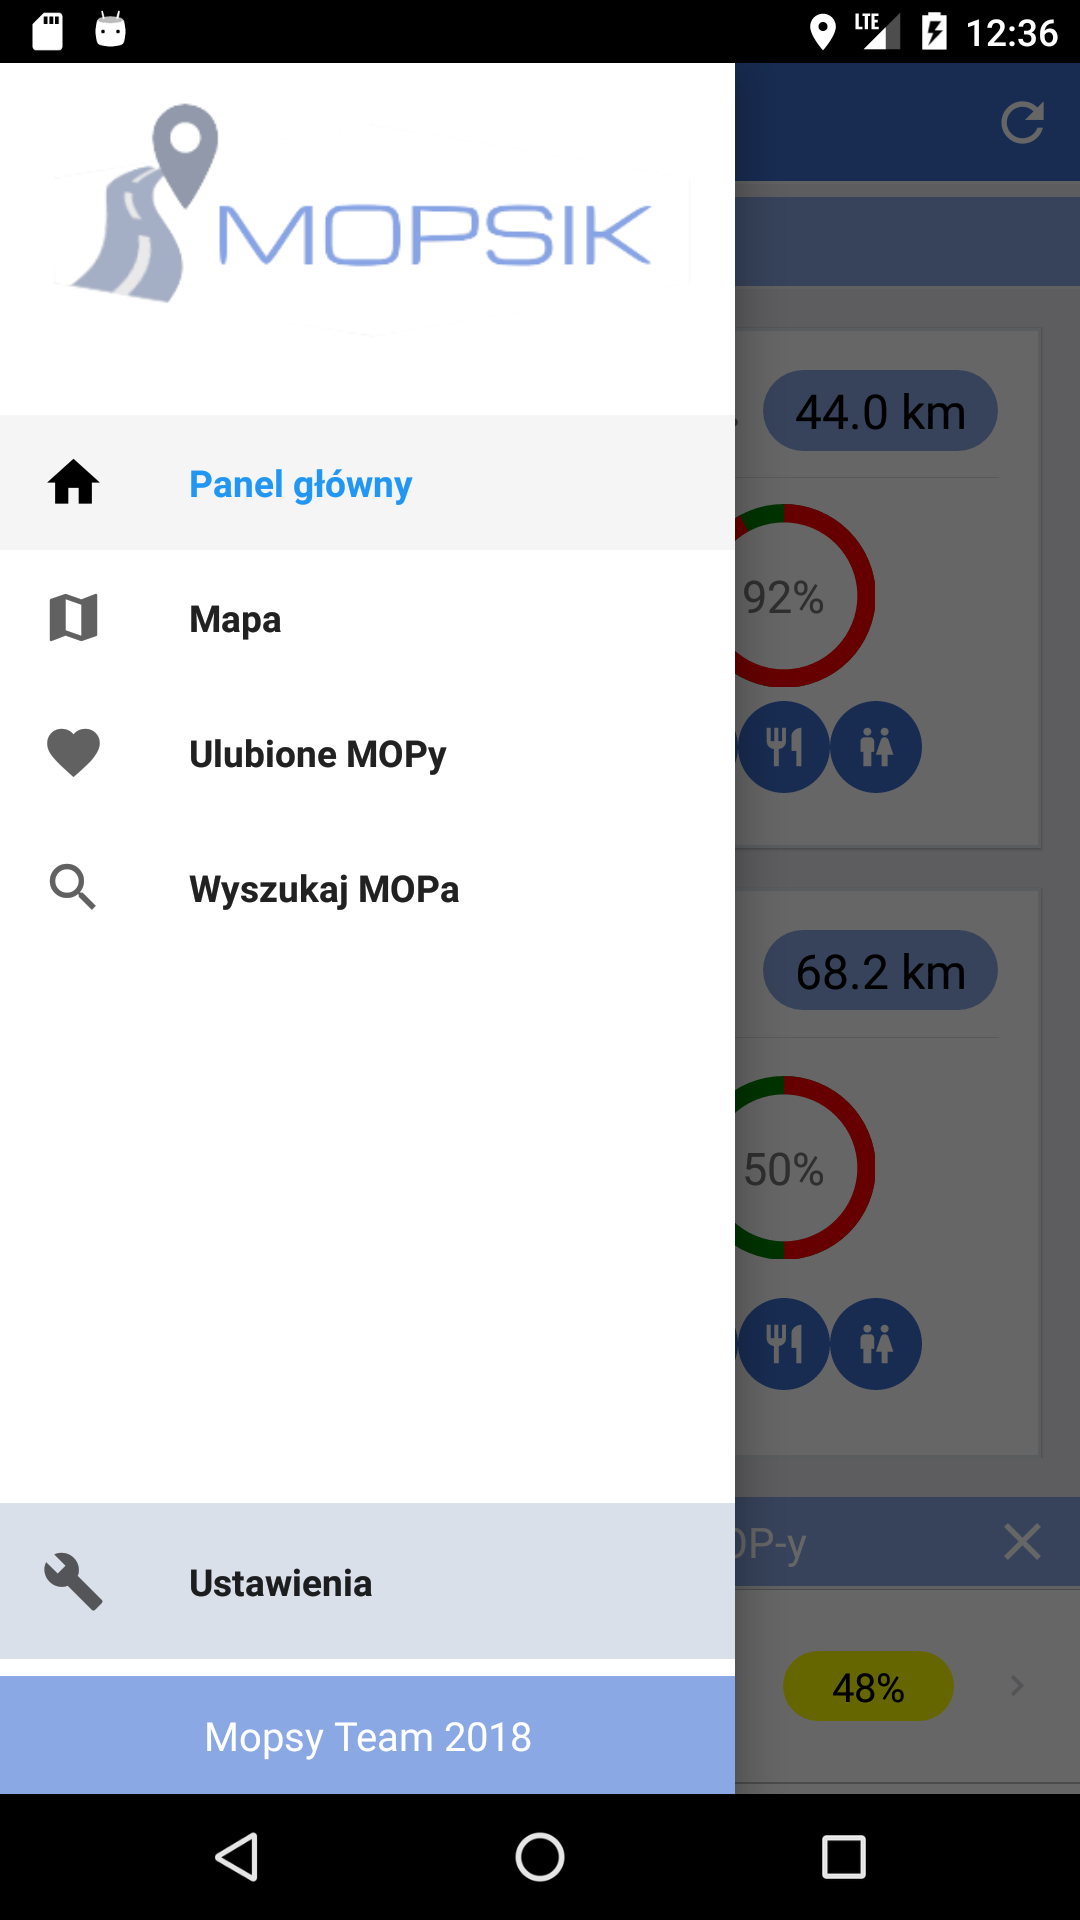
\includegraphics[width=5cm]{images/mopsik_mobile/menu.png}
  \captionof{figure}{Menu boczne}
  \label{mopsik_menu}
\end{minipage}
\end{figure}


\subsection{Konfiguracja aplikacji i ustawienia}
Przy pierwszym uruchomieniu aplikacji otwiera się panel konfiguracyjny, w którym należy ustawić dwa parametry:
\begin{enumerate}
\item \textit{Główny typ pojazdu} (pole jednokrotnego wyboru) -- w miejscach, w których znajdują się tylko ogólne informacje o MOP-ie wyświetlamy zajętość tylko dla głównego typu pojazdu
\item \textit{Wszystkie typy pojazdów} (pole wielokrotnego wyboru), którymi zainteresowany jest użytkownik -- w szczegółowych informacjach o MOP-ie wyświetlane są zajętości dla wszystkich zaznaczonych typów
\end{enumerate}
Typy pojazdów
\begin{enumerate}
\item Samochód osobowy
\item Samochód ciężarowy
\item Autobus
\end{enumerate}
Podział został wykonany w oparciu o zróżnicowane potrzeby użytkowników tych pojazdów, a także znaczące różnice w gabarytach, a co za tym idzie -- wymiarach potrzebnych miejsc parkingowych.
Konfigurację aplikacji można zmienić w każdej chwili w zakładce \emph{Ustawienia}.
W ustawieniach znajduję się także przycisk \textit{Zresetuj ustawienia}, który wymazuje z urządzenia wszystkie informacje zapisane przez aplikację i uruchamia ją ponownie. 

\begin{figure}[!htb]
\centering
\begin{minipage}{.5\textwidth}
  \centering
  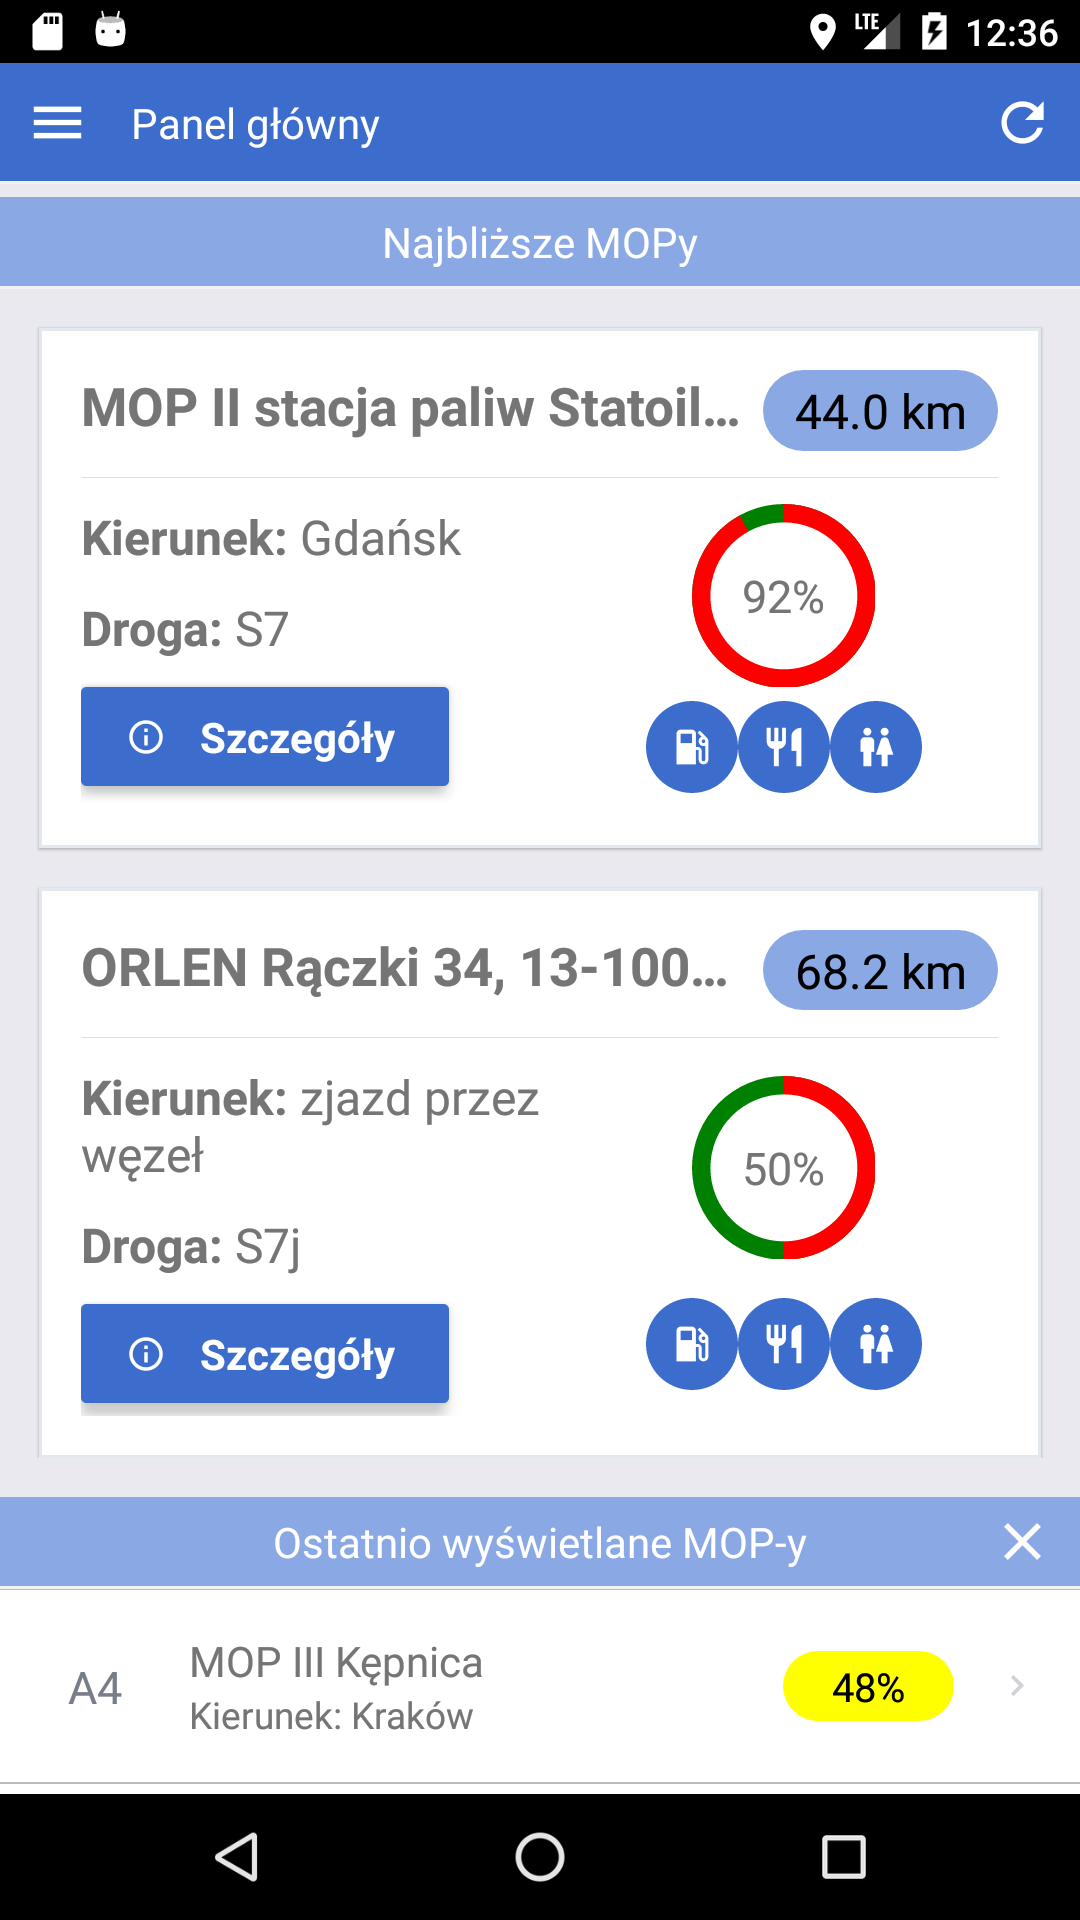
\includegraphics[width=5cm]{images/mopsik_mobile/home.png}
  \captionof{figure}{Panel główny}
  \label{mopsik_home}
\end{minipage}%
\begin{minipage}{.5\textwidth}
  \centering
  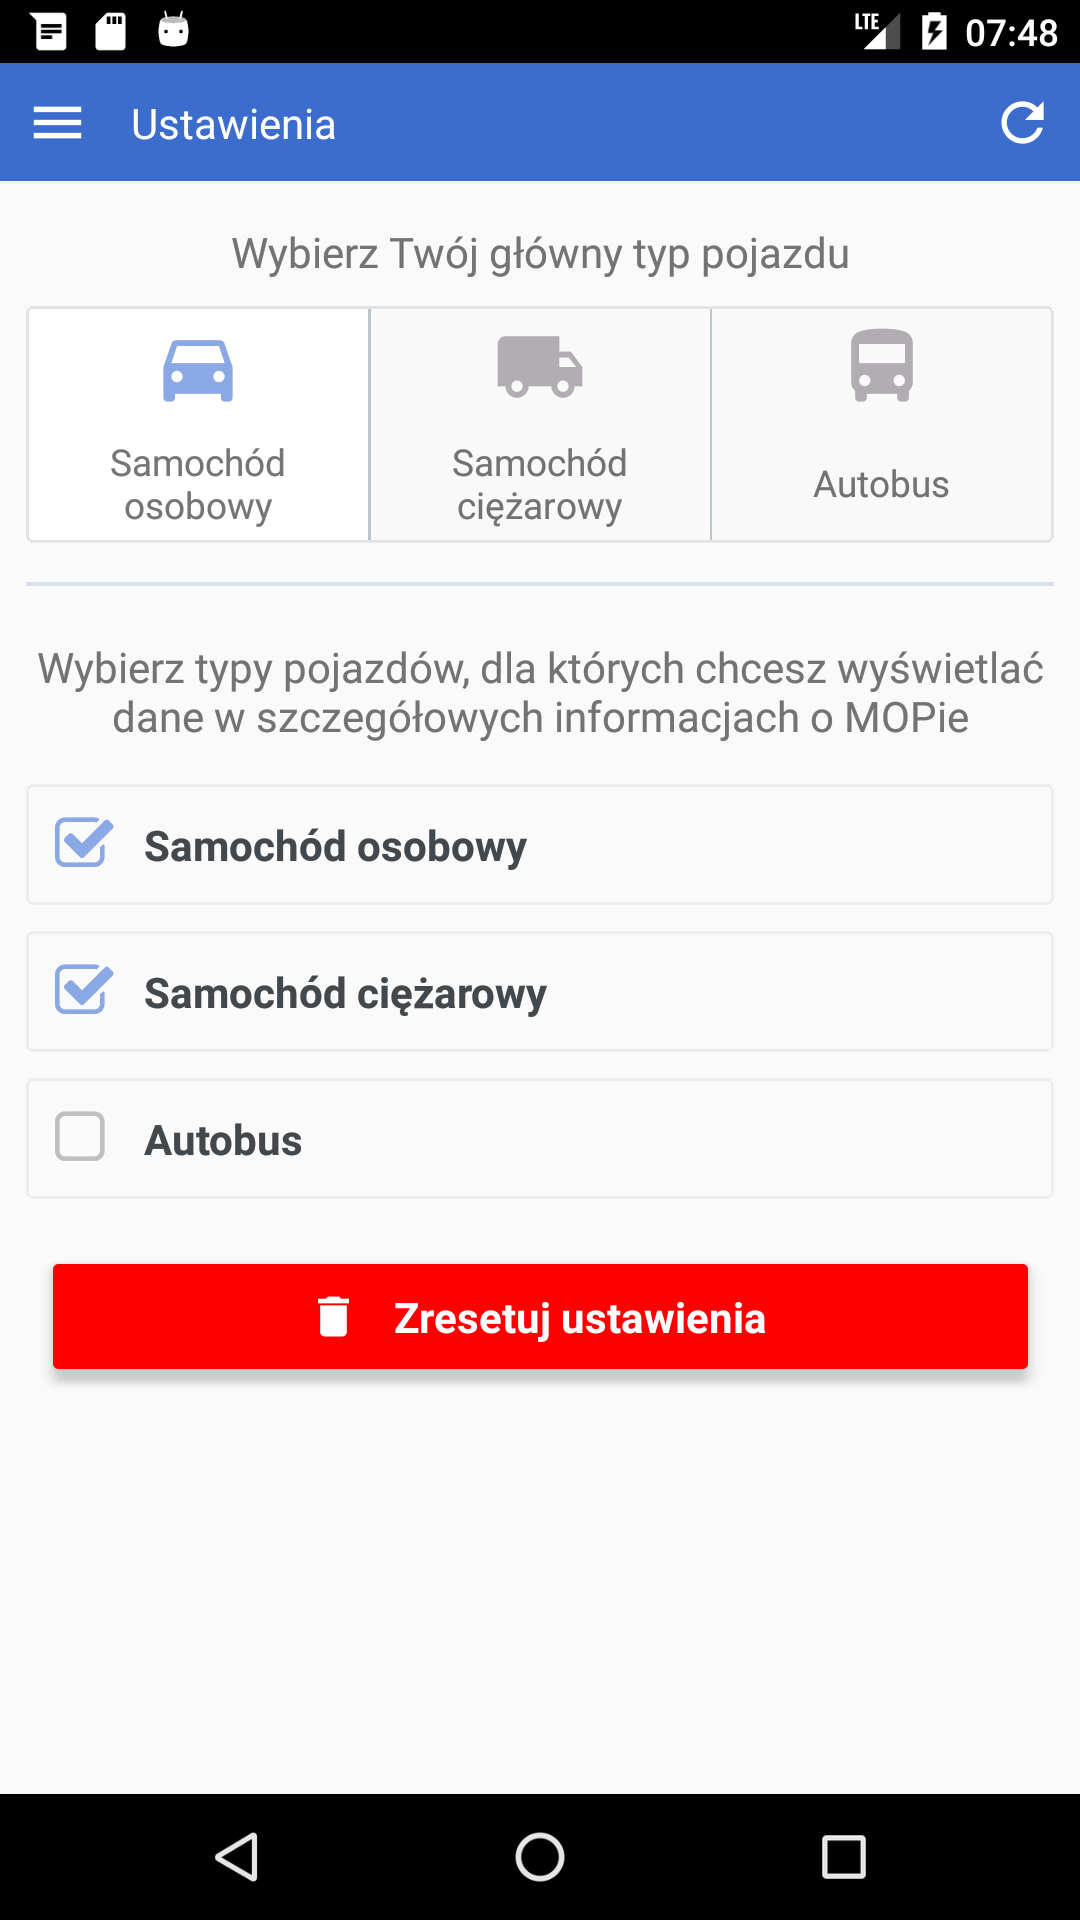
\includegraphics[width=5cm]{images/mopsik_mobile/settings.png}
  \captionof{figure}{Ustawienia}
  \label{mopsik_settings}
\end{minipage}
\end{figure}

\begin{figure}[!htb]
\centering
\begin{minipage}{.5\textwidth}
  \centering
  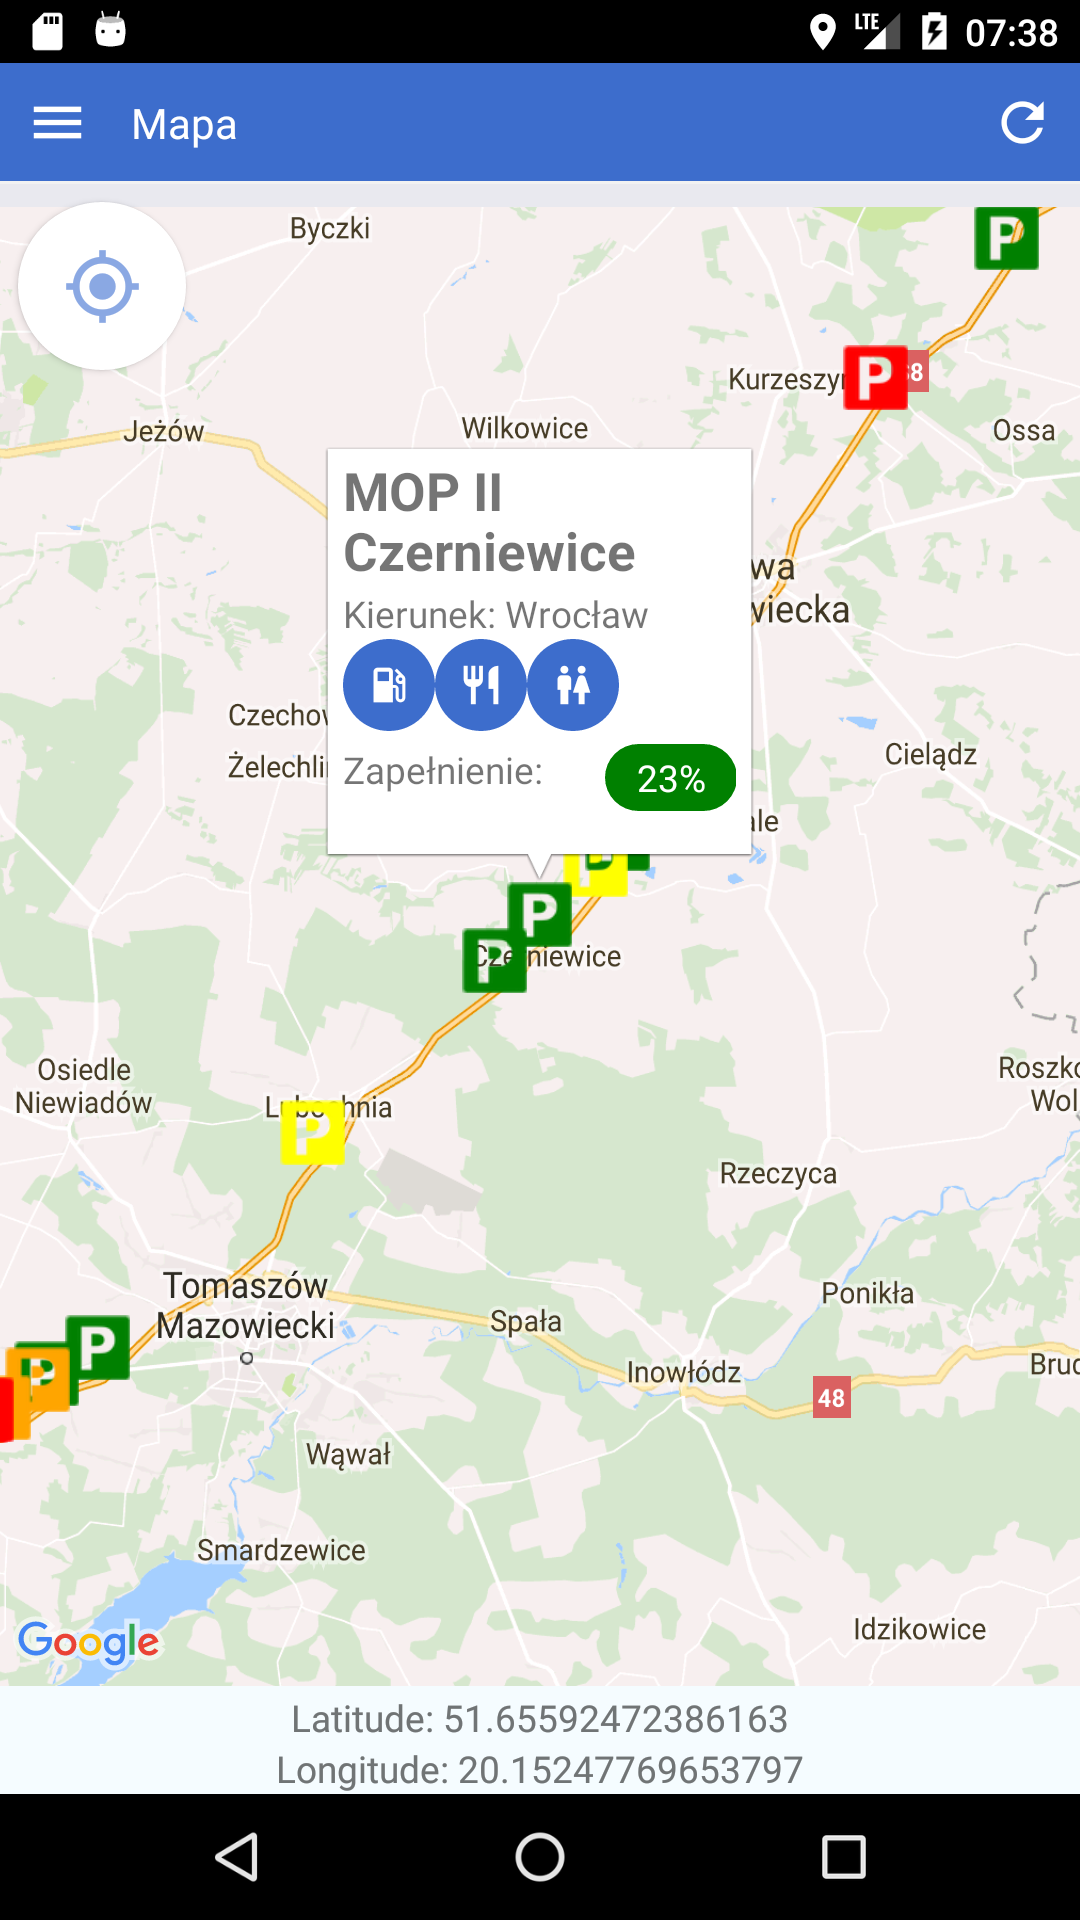
\includegraphics[width=5cm]{images/mopsik_mobile/map.png}
  \captionof{figure}{Mapa}
  \label{mopsik_map}
\end{minipage}%
\begin{minipage}{.5\textwidth}
  \centering
  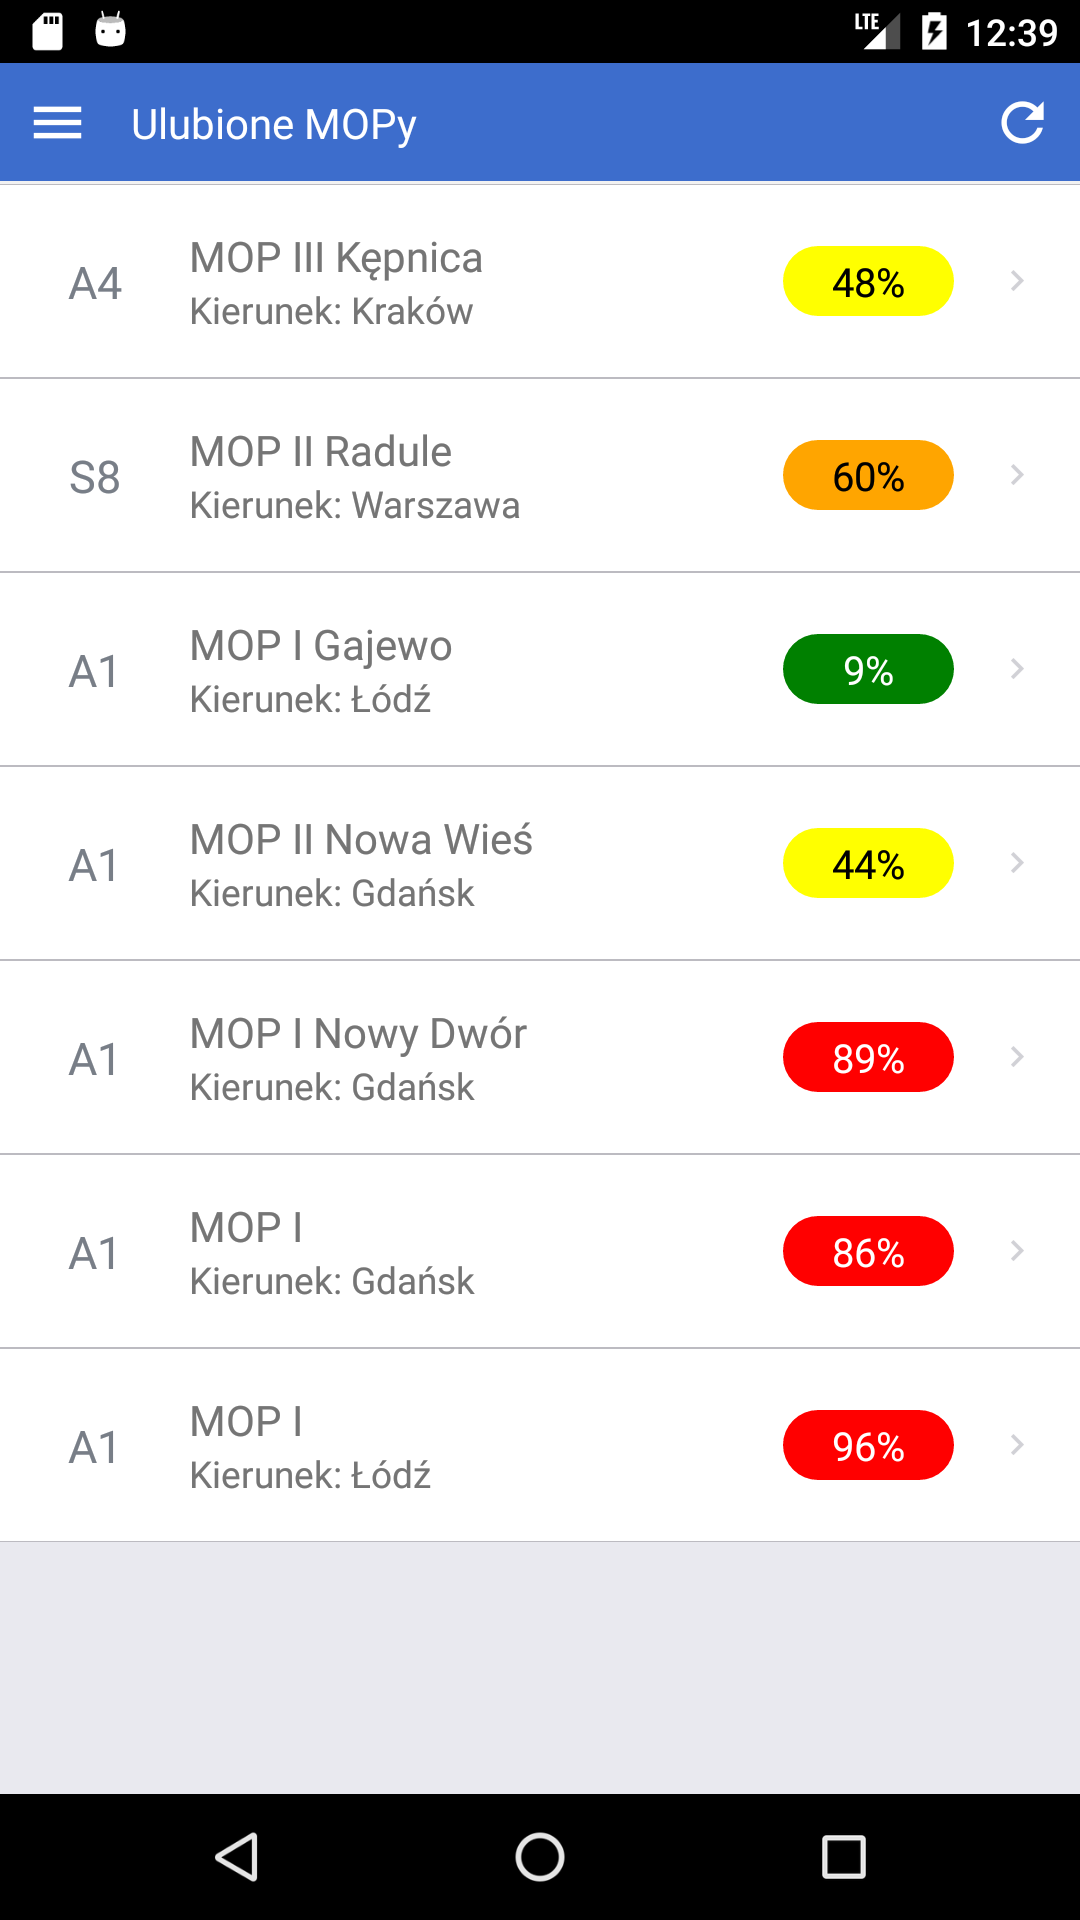
\includegraphics[width=5cm]{images/mopsik_mobile/favourites.png}
  \captionof{figure}{Ulubione}
  \label{mopsik_favourites}
\end{minipage}
\end{figure}

\begin{figure}[!htb]
\centering
\begin{minipage}{.5\textwidth}
  \centering
  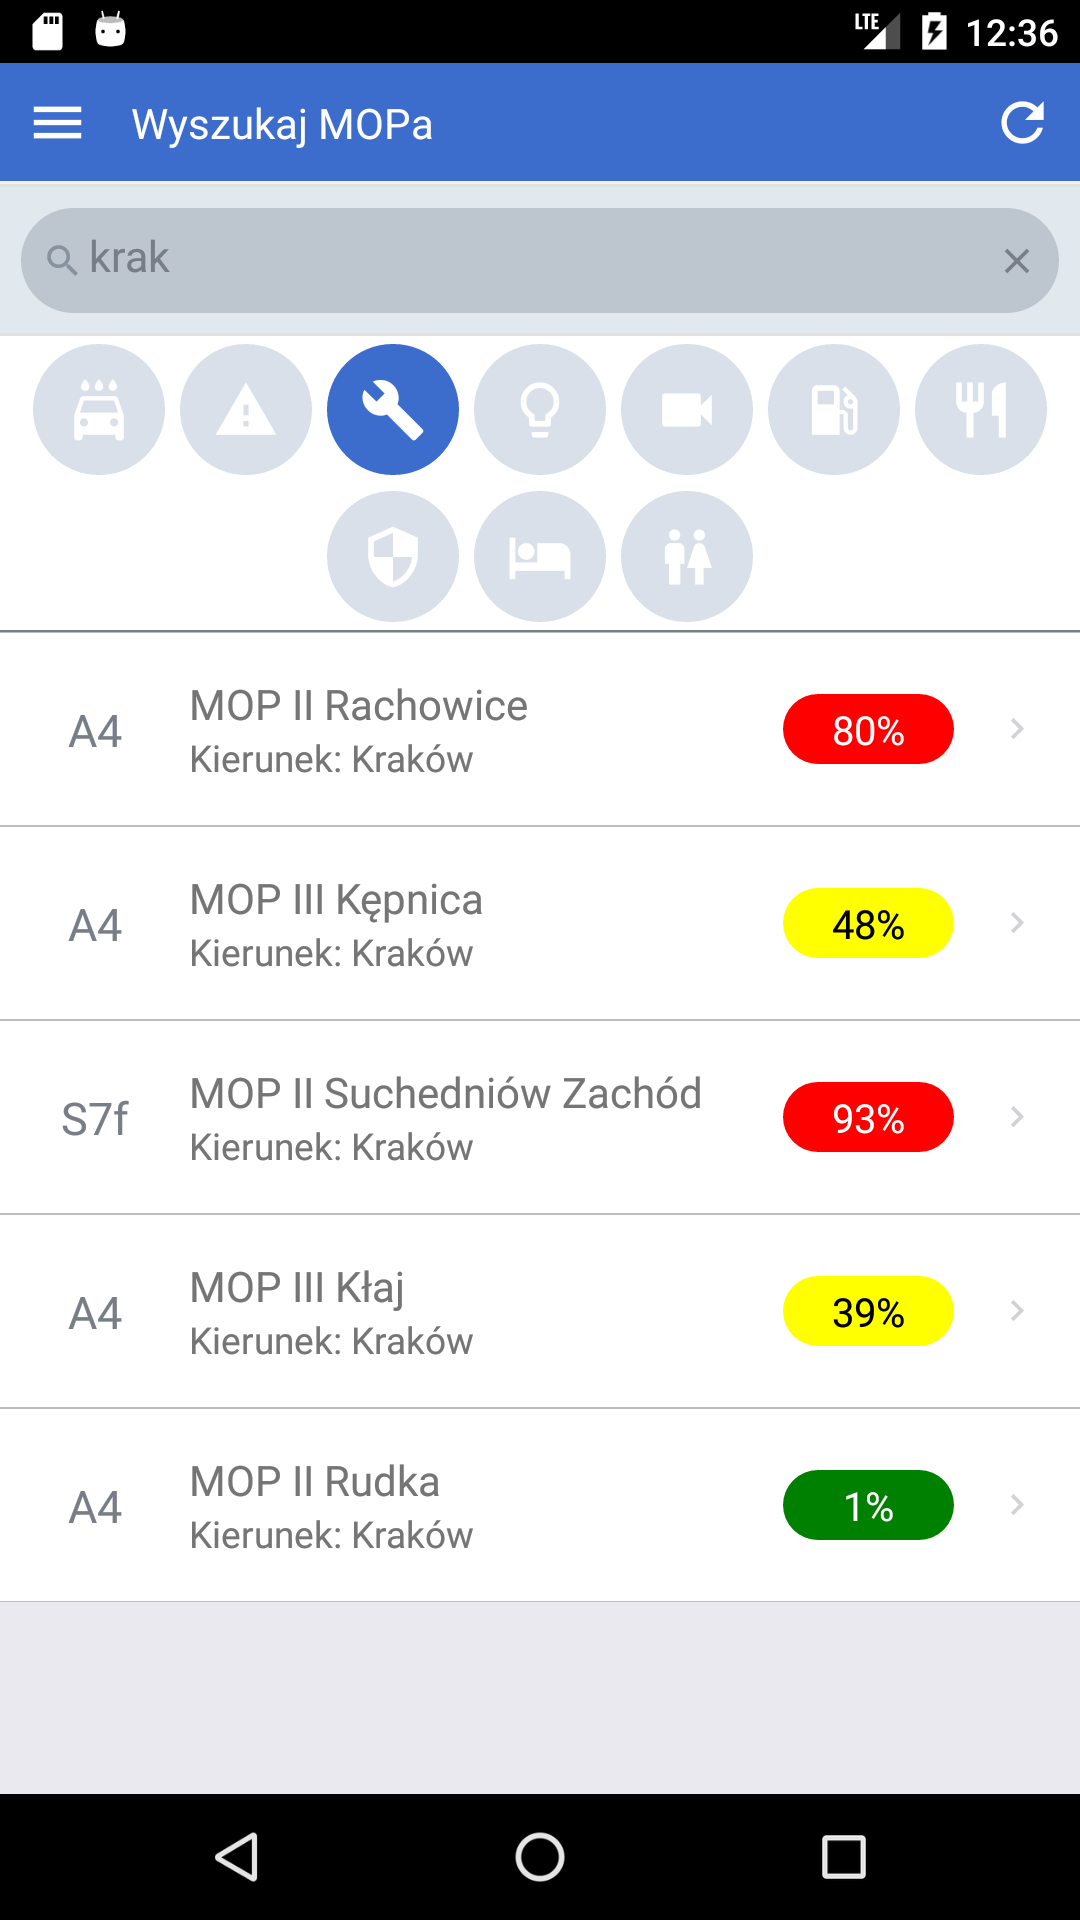
\includegraphics[width=5cm]{images/mopsik_mobile/search.png}
  \captionof{figure}{Wyszukiwarka}
  \label{mopsik_search}
\end{minipage}%
\begin{minipage}{.5\textwidth}
  \centering
  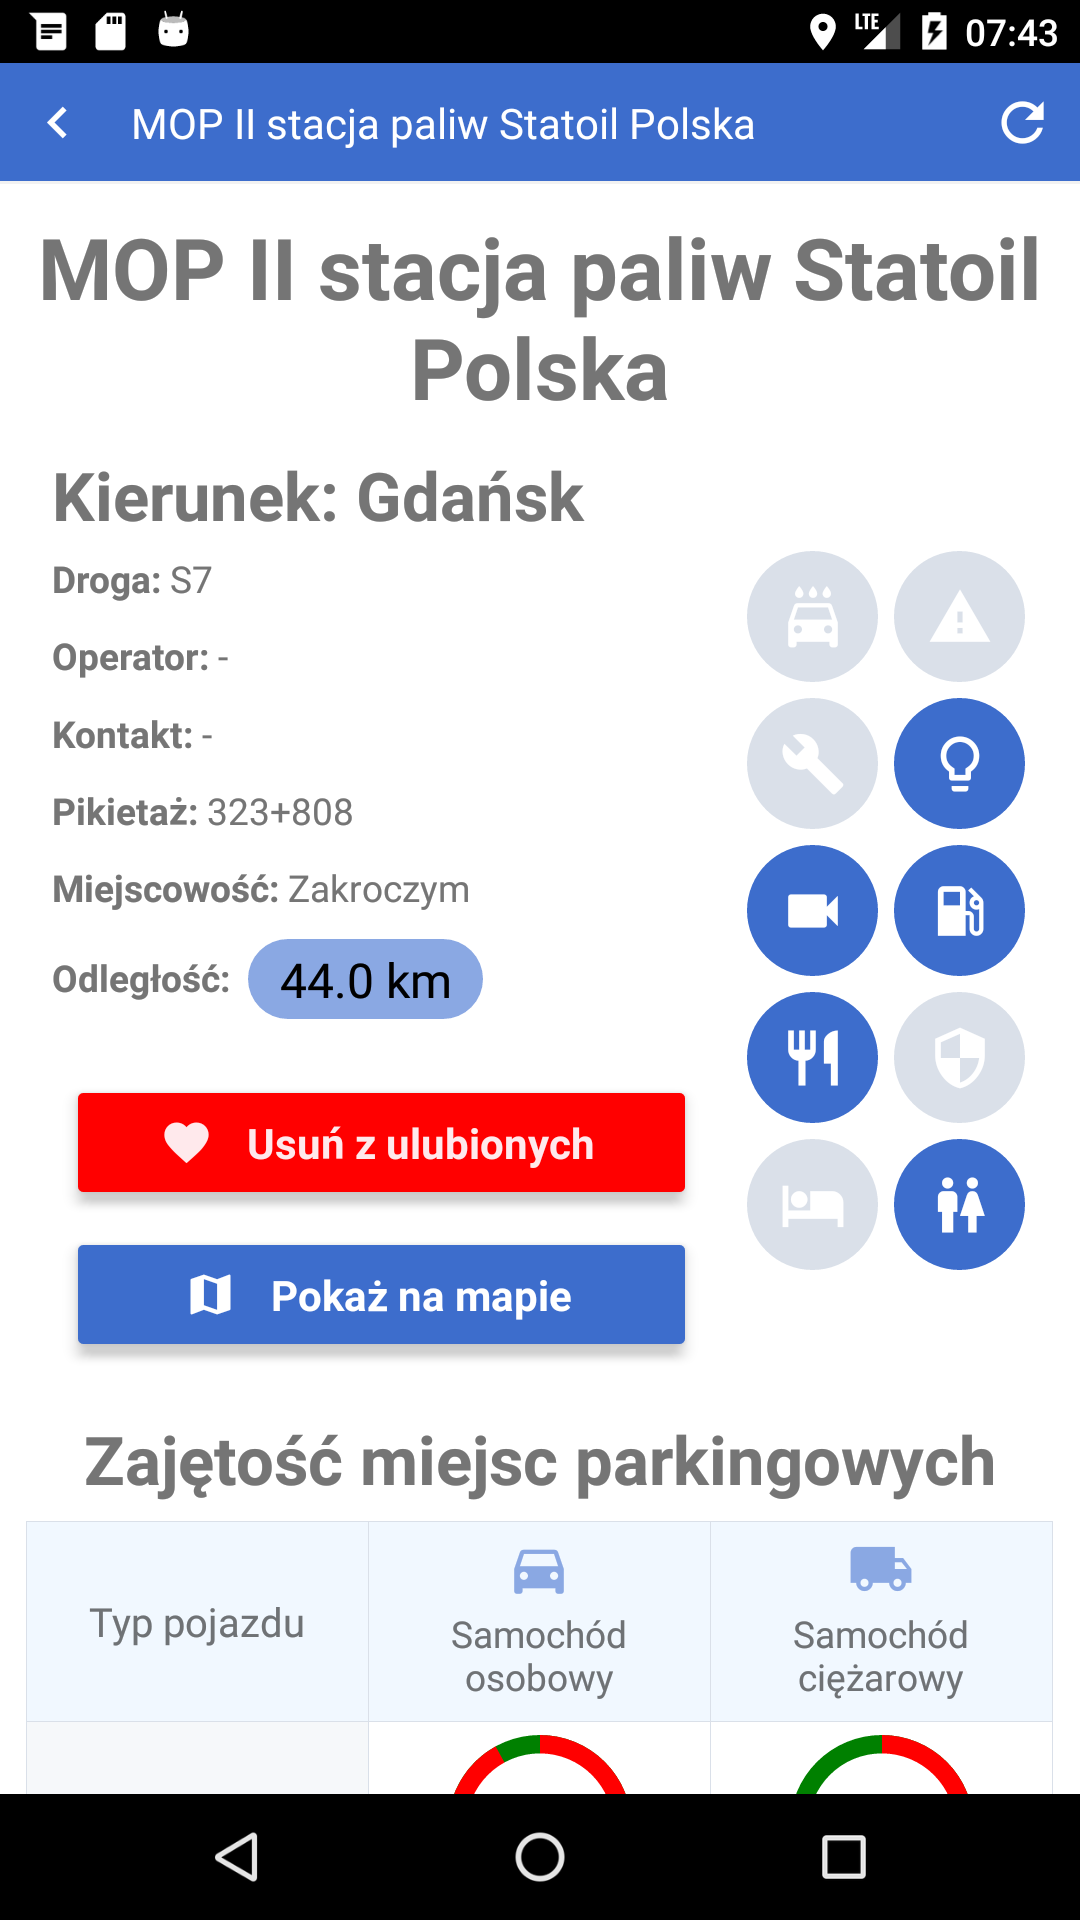
\includegraphics[width=5cm]{images/mopsik_mobile/details.png}
  \captionof{figure}{Szczegóły}
  \label{mopsik_details}
\end{minipage}
\end{figure}


\subsection{Google Maps}
\subsubsection{Warunki}
Jedną z podstawowych funkcji aplikacji Mopsik jest wyświetlanie mapy Polski z zaznaczonymi MOP-ami. Do tego celu wykorzystaliśmy Google Maps API. Dostęp do samej mapy i oznaczania na niej punktów jest nieodpłatny, dopóki aplikacja jest darmowa i ogólnodostępna\cite{google-api-faq}.
\subsubsection{Działanie}
Połączenie do API uwierzytelniane jest przez klucz wygenerowany na stronie \url{https://console.developers.google.com/apis/credentials}. Z każdym przeładowaniem widoku z mapą do~API wysyłane jest zapytanie z prośbą o konkretny fragment mapy świata, który jest zwracany w odpowiedzi, a następnie wyświetlany w aplikacji. Na mapie znajdują się markery oznaczające MOP-y. Kolor markera jest uzależniony od zajętości MOP-a dla wybranego \textit{głównego typu pojazdu}. Aplikacja wyświetla aktualną lokalizację użytkownika oraz umożliwia jej śledzenia (mapa porusza się wraz z użytkownikiem). 
\subsubsection{Wydajność}
Dodawanie markerów na mapie, a szczególnie tych z własną ikoną, znacząco obniża wydajność mapy. Aby ją poprawić zastosowaliśmy kilka zabiegów:
\begin{enumerate}
\item Do mapy dodawane są tylko markery znajdujące się w obecnie widocznym obszarze. Wraz z przesuwaniem mapy ładowane są kolejne.
\item Mapa przeładowywana jest nie częściej niż co 2 sekundy. Zapobiega to ciągłemu odświeżaniu gdy odczyty GPS urządzenia są niedokładne i nieprzerwanie drgają.
\item Wykorzystanie \textit{onRegionChangeComplete} zamiast \textit{onRegionChange} -- obie funkcje wywoływane są gdy użytkownik porusza mapą, czyli przy zmianie aktualnie widocznego fragmentu. \textit{onRegionChangeComplete} wywoływane jest tylko raz -- po zakończonym przeciągnięciu. Animacje są nieco mniej płynne, ale aplikacja nie zawiesza się przez ciągłe przeładowywanie mapy i znaczników MOP-ów.
\end{enumerate}
\subsubsection{Bezpieczeństwo}
Śledzenie lokalizacji użytkownika jest realizowane dzięki geolokazji urządzenia przenośnego -- mapy Google nie biorą w niej udziału. Zapytanie wysyłane do Google zawierają jedynie obszar (wpsółrzędne środa oraz przybliżenie), dla którego chcemy wyświetlić mapę. Jeżeli użytkownik aktywuje podążanie mapy za jego aktualnym położeniem, siłą rzeczy zapytania API będą wysyłać jego kolejne lokalizacje. Jednak zakładając korzystanie z map online -- nie ma innej możliwości. 

\subsection{Zapytanie do API}
Po otwarciu aplikacji wykonywane jest zapytanie do \acrshort{api} \textit{/mops}, które zwraca wszystkie informacje o MOP-ach. Dane te są przetwarzane i zapamiętywane.
Po wciśnięciu przycisku \textit{odśwież} oraz po otwarciu każdej z zakładek, wykonywane jest zapytanie \textit{/taken} zwracające tylko aktualną liczbę zajętych miejsc parkingowych dla każdego z MOP-ów. Aplikacja aktualizuje te dane w zapisanych MOP-ach oraz przelicza nowe zajętości dla wszystkich typów pojazdów.
Do każdego typu pojazdu, w każdym MOP-ie, przyporządkowywany jest kolor zgodnie z ustaloną legendą (np. dla małej zajętości, do 30\% -- zielony, a dla największej -- czerwony). Ten kolor jest następnie wykorzystywany przy wizualizacji danych.

\subsection{Użyte biblioteki}
W aplikacji skorzystaliśmy z gotowych bibliotek \acrshort{rn}, co znacząco przyspieszyło i~ułatwiło pracę.
\begin{enumerate}
\item \textbf{lodash} \\
\url{https://www.npmjs.com/package/lodash}\\
Dostarcza funkcji użytkowych w paradygmacie funkcyjnym. Przydatna w mapowaniu MOP-ów.

\item \textbf{react-native-elements}\\
\url{https://react-native-training.github.io/react-native-elements/}\\ 
Biblioteka zawierająca wiele gotowych komponentów. Skorzystaliśmy m.in. z \textit{Drawer} (menu boczne), \textit{Header} (nagłówek) i \textit{SearchBar} (wyszukiwarka).

\item \textbf{react-native-maps} \\
\url{https://github.com/react-community/react-native-maps}\\
Biblioteka umożliwiająca połączenie do Google Maps API i renderowanie map.

\item \textbf{react-native-restart} \\
\url{https://github.com/avishayil/react-native-restart}\\
Biblioteka umożliwia restart aplikacji z poziomu kodu. Wykorzystana przy resetowaniu ustawień.

\item \textbf{react-native-svg} \\
\url{https://github.com/react-native-community/react-native-svg}\\
Służy do grafiki wektorowej.

\item \textbf{react-native-svg-circular-progress} \\
\url{https://github.com/stssoftware/react-native-svg-circular-progress}\\
Wykorzystana do rysowania wykresów zajętości MOP-ów. Wymaga bibkioteki \textit{react-native-svg}.

\item \textbf{react-native-swipeout} \\
\url{https://github.com/dancormier/react-native-swipeout}\\
Umożliwia dodawanie przycisków pojawiających się po przesunięciu w bok komponentu. W naszej aplikacji odpowiada za pojawianie się przycisku \textit{Usuń} na liście ulubionych MOP-ów.

\item \textbf{react-native-table-component} \\
\url{https://github.com/Gil2015/react-native-table-component}\\
Generuje tabelę z liczbą wolnych miejsc parkingowych w zakładce \textit{Szczegółowe informacje o MOP-ie}.

\item \textbf{react-native-vector-icons} \\
\url{https://github.com/oblador/react-native-vector-icons}\\
Dostęp do ikon z \url{https://material.io/icons/}.

\item \textbf{react-navigation} \\
\url{https://reactnavigation.org}\\
Otoczka całej aplikacji. Odpowiada za nawigowanie wewnątrz aplikacji i poruszanie pomiędzy widokami.
\end{enumerate}

\subsection{Nawigacja}
W aplikacji wykorzystaliśmy dwa typy nawigacji - stos (\textit{StackNavigator}) i menu boczne (\textit{DrawerNavigator}). Architektura nawigacji została przedstawiona na rysunku \ref{mopsik_nav}.\\


Najbardziej zewnętrznym elementem aplikacji jest komponent \textit{DrawerNavigator}. Dodany jest do niego widok \textit{SettingsView}, a także stosy \textit{HomeStack}, \textit{MapStack}, \textit{FavouritesStack} i \textit{SearchStack}. Menu boczne jest utworzone przez dostosowany do naszych potrzeb komponent \textit{DrawerContent} -- dodane zostało logo i autorzy. \\

Z zakładek \textit{Home}, \textit{Ulubione}, \textit{Wyszukiwarka} i \textit{Mapa} można przejść do widoku \textit{MopDetailsView}, a stamtąd do \textit{MapView} w trybie \textit{Pokaż MOP-a na mapie} (focused). Za tą część nawigacji odpowiedzialny jest \textit{StackNavigator}. Bedąc w szczegółowych informacjach o MOP-ie i skupionej mapie w nagłówku pojawia się przycisk cofania.\\

Komponenty Stack obudowują nawigację stosową. Wewnątrz każdego ze stosów można poruszać się po trzech widokach - głównym, szczegółowym i mapie (wyśrodkowanej na wybranym MOP-ie, z otwartym dymkiem). W widokach głównych (tj. domowym, mapie, wyszukiwarce i ulubionych) widoczne są listy wielu MOP-ów. Po kliknięciu w wybrany MOP, aplikacja przenosi do widoku ze szczegółami wraz z odpowiednim parametrem. Na jego podstawie renderowane są informacje o tym wybranych MOP-ie. Ze szczegółów można poprzez kliknięcie w przycisk \textit{Pokaż na mapie} przejść do \textit{MapView} -- o ile wcześniej nie przyszliśmy z mapy. \newline Czyli nie jest możliwe poruszanie się\\	\indent mapa --> szczegóły(A) --> mapa --> szczegóły(B) -/-> mapa --> ... ,\\ponieważ w widoku szczegóły(B) nie pojawia się przycisk \textit{Pokaż na mapie}.


\begin{figure}[!htb]
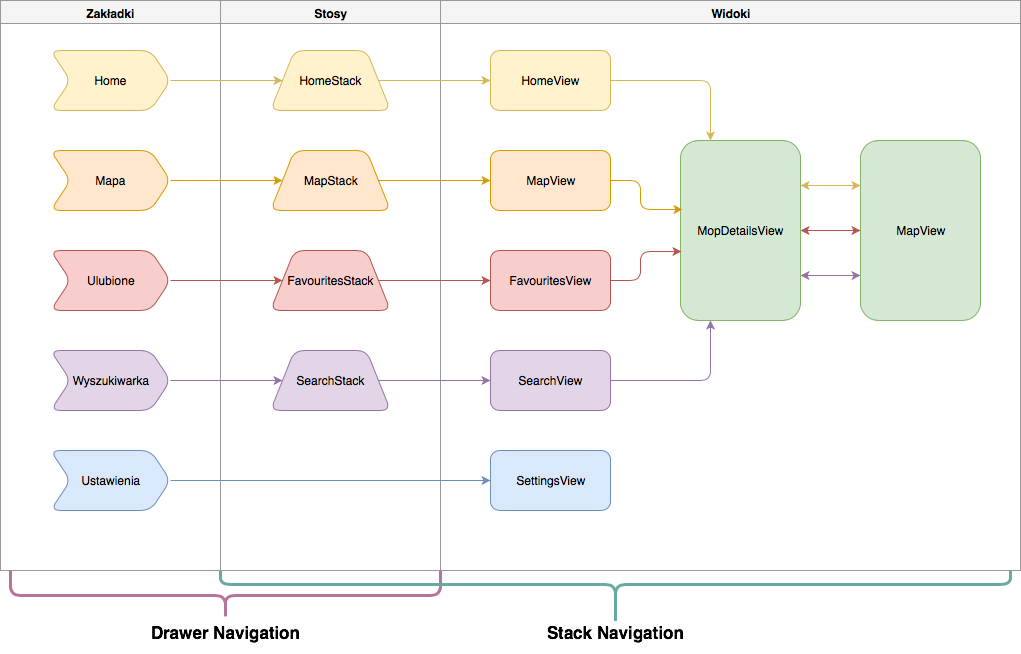
\includegraphics[width=\textwidth]{images/mopsik_mobile_navigation.png}\label{mopsik_nav}
\caption{Schemat nawigacji aplikacji mobilnej Mopsik}
\end{figure}

\subsection{Pozostałe komponenty}
Na rysunku \ref{mopsik_mobile_structure} przedstawiona została struktura plików Mopsika. Poza komponentami opisanymi w poprzednim punkcie, aplikacja korzysta z narzędzi znajdujących się folderze \textit{tools}.
\begin{enumerate}
\item \textit{DrawerContent} -- menu boczne
\item \textit{Header} -- nagłówek
\item \textit{LastViewedMops} -- komponent wyświetlający do trzech ostatnio wyświetlanych MOP-ów
\item \textit{MopListItem} -- element listy wyświetlający nazwę, drogę, kierunek i zajętość dla głównego typu pojazdu; wykorzystywany w \textit{Ulubionych}, \textit{Wyszukiwarce} i \textit{Ostatnio wyświetlanych}
\item \textit{NearestMops} -- komponent wyświetlający dwa MOP-y znajdujące się najbliżej aktualnej lokalizacji użytkownika
\item \textit{SplashScreen} -- ekran powitalny; w trakcie jego wyświetlania aplikacja pobiera dane o MOP-ach z api oraz zapisane informacje z AsyncStorage
\item \textit{SubHeader} -- nagłówek sekcji; używany w ekranie domowym
\item \textit{UsageCircle} -- wykres kołowy zajętości miejsc parkingowych
\item \textit{UsageTable} -- tabela z liczbą i zajętością miejsc parkingowych dla typów pojazdów wybranych w ustawieniach
\end{enumerate}
\begin{figure}[!htb]
\caption{Struktura plików aplikacji mobilnej Mopsik}
\dirtree{%
.1 mopsik mobile.
.2 src.
.3 components.
.4 stacks.
.5 FavouritesStack.js.
.5 HomeStack.js.
.5 MapStack.js.
.5 SearchStack.js.
.4 tools.
.5 DrawerContent.js.
.5 Header.js.
.5 LastViewedMops.js.
.5 MopListItem.js.
.5 NearestMops.js.
.5 SplashScreen.js.
.5 SubHeader.js.
.5 UsageCircle.js.
.5 UsageTable.js.
.4 views.
.5 FavouritesView.js.
.5 HomeView.js.
.5 MapView.js.
.5 MopDetailsView.js.
.5 SearchView.js.
.5 SettingsView.js.
.3 config.
.4 facilities.js.
.4 favourites.js.
.4 findNearestMop.js.
.4 mops.js.
.4 settings.js.
.4 styles.js.
.4 themes.js.
.4 vehicles.js.
.3 images.
.4 ....
.2 ....
}\label{mopsik_mobile_structure}
\end{figure}



\subsection{Pliki konfiguracyjne i funkcje}
W folderze \textit{config} znajdują się pliki, w których zdefiniowane są dane statyczne oraz funkcje odpowiedzielne za przetwarzanie danych.
\begin{enumerate}
\item \textit{facilities} -- zdefiniowane usługi dostępne na MOP-ach, odpowiadające im polskie nazwy oraz ikony, funkcje generujące komplet ikon do wyświetlania w informacjach o MOP-ie
\item \textit{favourites} -- funkcje odpowiedzialne za pobieranie MOP-ów zapisanych do ulubionych, zapisywanie, usuwanie
\item \textit{findNearestMop} -- funkcja, która po otrzymaniu współrzędnych punktu, zwraca dwa MOP-y znajdujące się najbliżej tego punktu oraz odległości do niego w kilometrach
\item \textit{mops} -- funkcje pobierające informacje o MOP-ach z API, dobierające kolory według legendy
\item \textit{settings} -- plik ze zmiennymi przechowującymi ustawienia aplikacji
\item \textit{styles} -- zdefiniowane style komponentów
\item \textit{themes} -- zdefiniowane motywy kolorystyczne
\item \textit{vehicles} -- typy pojazdów wraz z polskimi nazwami i ikonami
\end{enumerate}

\subsection{Zapisywanie danych}
Podczas działania aplikacji dane zapisywane są w zmiennych znajdujących się m.in. w plikach mops.js i settings.js. Można nazwać je pseudoglobalnymi, ponieważ ich wartość można zmieniać w każdym kompomencie, o ile zostały odpowiednio zaimportowane. Informacje te są tracone wraz z zamknięciem aplikacji.\\
Dane dotyczące ustawień użytkownika oraz ulubionych MOP-ów nie znikają. Do tego celu wykorzystujemy AsyncStorage. Dane pobierane i zapisywane są asynchronicznie. Zasób ma postać słownika -- każda wartość znajduje się pod nadanym jej kluczem.


\chapter{Mopsik -- Strona internetowa}

\section{Przypadki użycia}
Przypadki użycia strony internetowej \textit{Mopsik} zostały przedstawione w poprzednim rozdziale, razem z przypadkami użycia aplikacji mobilnej.

\section{Architektura i opis implementacji}

\subsection{Technologia}
\begin{figure}[!htb]
    \centering
    \begin{minipage}{.7\textwidth}
Aplikacja internetowa została napisana w technologii ASP.NET MVC, w języku obiektowym C\#. Frontend wykorzystuje także HTML, JavaScript oraz CSS. W aplikacji znajdują się trzy kontrolery odpowiedzialne za poszczególne elementy: Mapa, Wyszukiwarka, Szczegóły. W każdym kontrolerze zdefiniowane są akcje. Na podstawie aktualnego adresu wywoływany jest odpowiedni kontroler i akcja:\\ \textit{<domena>/<nazwa kontrolera>/<nazwa akcji>/<parametry>}.
    \end{minipage}%
    \begin{minipage}{.3\textwidth}
        \centering
        
\includegraphics[width=5cm]{images/mvc.png}\label{MVC_logo}
    \end{minipage}
\end{figure}

\subsection{Zakładki}
W górnej części strony znajduje się menu, w którym są dwie zakładki: \textit{Mapa} i \textit{Wyszukiwarka}. \textit{Mapa} jest zakładką domyślną. Jest także trzeci widok -- \textit{Szczegóły}, do którego można przejść z obu zakładek, po wyborze jednego z MOP-ów.
\subsubsection{Mapa}
W tej zakładce znajduje się mapa Polski z OpenStreetMap. Do jej wyświetlania wykorzystane zostały OpenLayers - biblioteka JavaScript do dynamicznych map. Na mapie oznaczone są MOP-y, a kolor znacznika odpowiada zajętości miejsc parkingowych dla wybranego typu pojazdu (skala analogiczna jak w aplikacji mobilnej). Typ pojazdu można zmienić w prawym, górnym rogu mapy, wybierając odpowiednią ikonę. Wysyła to zapytanie POST z odpowiednią wartością typu pojazdu i odświeża stronę z naniesionymi zmianami. 
Po kliknięciu w znacznik wyświetla się dymek z podstawowymi informacjami o MOP-ie, a guzik z ikoną informacji przenosi do szczegółów -- wywołuje \textit{DetailsController} z akcją \textit{Details} oraz parametrem id MOP-a.

\begin{figure}[!htb]
\centering
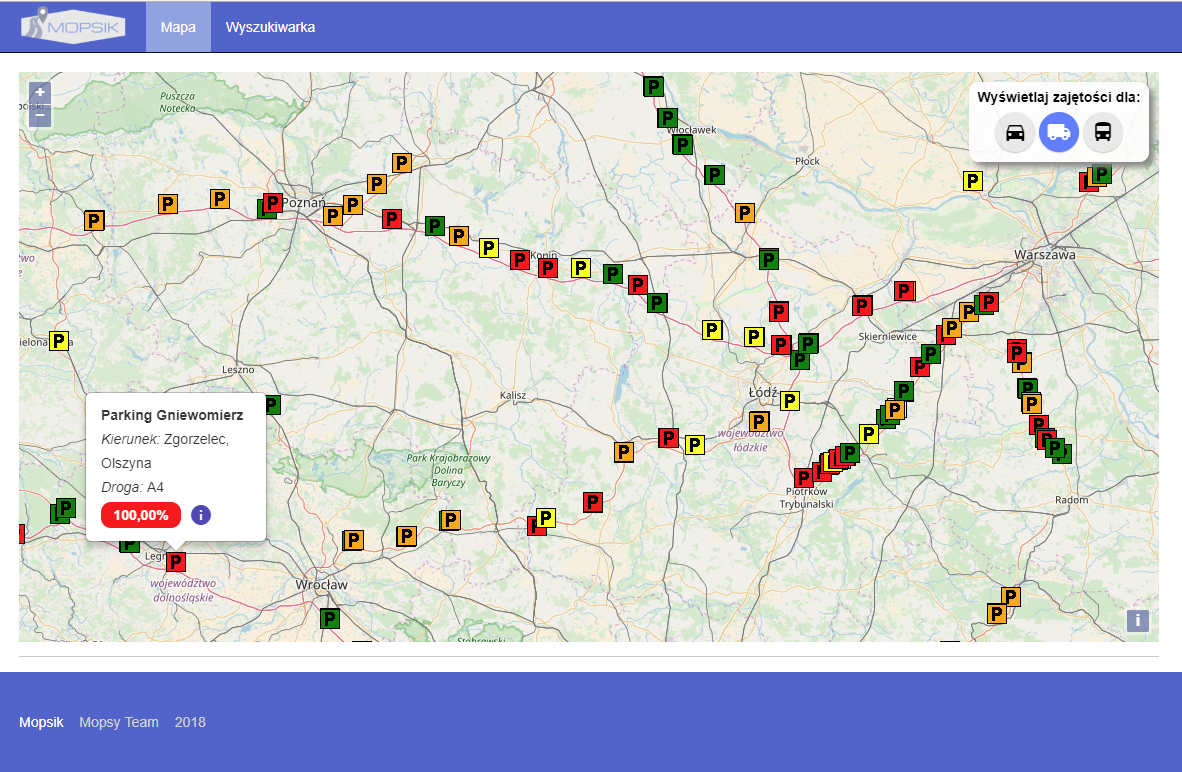
\includegraphics[width=\textwidth]{images/mopsik_www/map.png}
\captionof{figure}{Mapa}
\label{mopsik_www_map}
\end{figure}

\subsubsection{Wyszukiwarka}
Aplikacja umożliwia wyszukiwanie MOP-ów po nazwie, miejscowości, numerze drogi i kierunku oraz filtrowanie po obecnych usługach. Przyciski \textit{Szukaj} i \textit{Filtruj} wysyłają zapytanie POST wraz z aktualną frazą wyszukiwania i zaznaczonymi usługami.
Wyszukiwarka posiada \textit{form} z polem \textit{input} na wyszukiwany tekst oraz ukrytym polem \textit{input}, które przesyła aktualnie zaznaczone filtry. W formularzu odpowiadającym za filtrowanie jest odwrotnie.  
MOP uznawany jest za pasujący do zapytania jeśli:
\begin{enumerate}
\item oferuje wszystkie usługi zaznaczone w filtrach
\item dla każdego ze słów zawartych w wyszukiwanym haśle, MOP zawiera to słowo w jednym z poniższych:
\begin{enumerate}
\item nazwa
\item miejscowość
\item numer drogi
\item kierunek
\end{enumerate}
(wielkość liter nie jest istotna)
\end{enumerate}
W liście rezultatów znajdują się wszystkie MOP-y, które spełniają warunki zapytania. Dla każdego z nich wyświetlane są: nazwa, numer drogi, kierunek, miejscowość oraz zajętość dla wszystkich trzech typów pojazdów. Kliknięcie w wiersz z MOP-em przenosi na stronę ze szczegółami.

\begin{figure}[!htb]
\centering
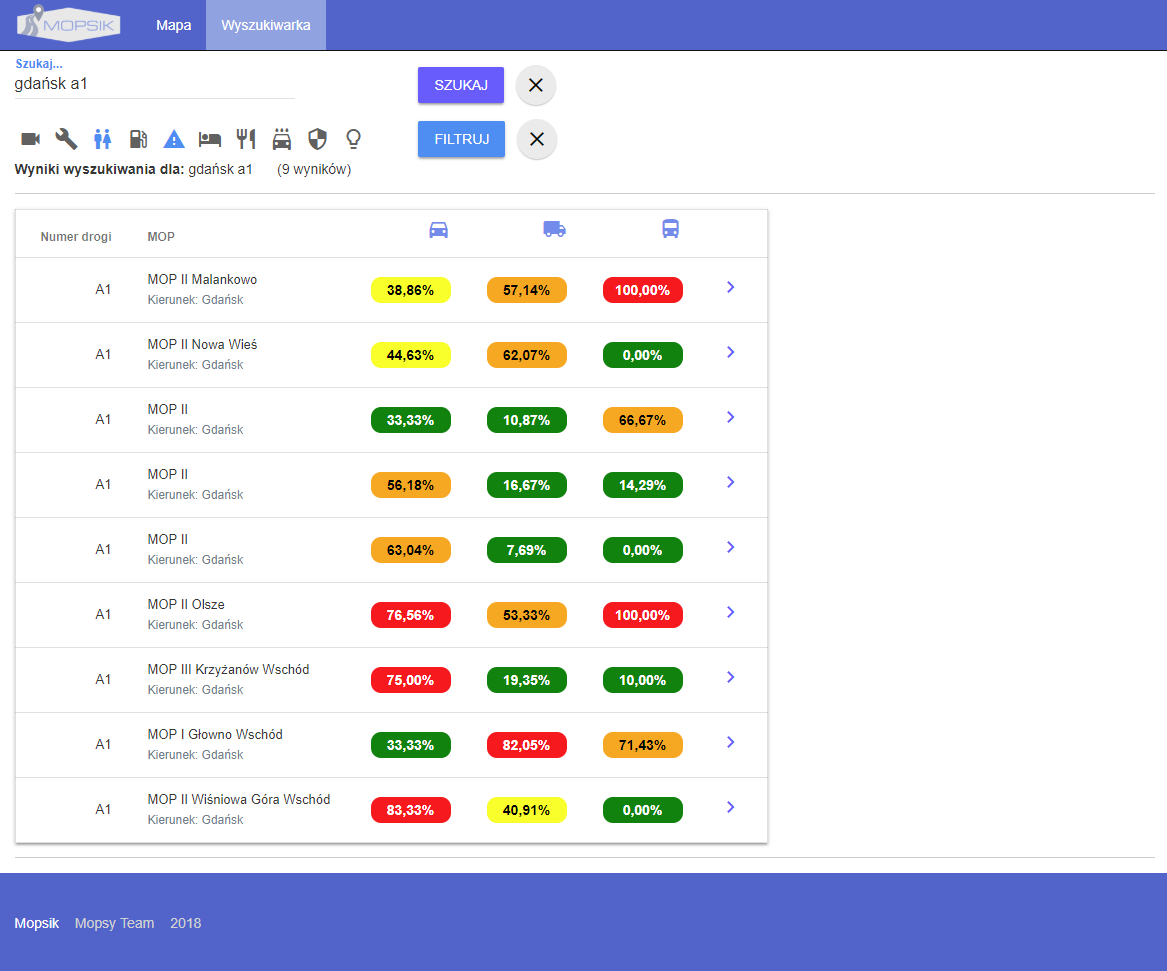
\includegraphics[width=\textwidth]{images/mopsik_www/search.png}
\captionof{figure}{Wyszukiwarka}
\label{mopsik_www_search}
\end{figure}

\subsubsection{Szczegóły}
W tej zakładce wyświetlane są szczegółowe informacje o konkretnym MOP-ie:
\begin{enumerate}
\item nazwa
\item kierunek
\item numer drogi
\item miejscowość
\item pikietaż
\item współrzędne geograficzne
\item operator i kontakt do niego -- numer telefonu oraz e-mail
\item oferowane usługi
\item położenie ma napie
\item dla każdego typu pojazdu:
\begin{enumerate}
\item zajętość miejsc parkingowych w procentach + wizualizacja danych na wykresie
\item liczba wolnych miejsc parkingowych
\item liczba zajętych miejsc parkingowych
\item liczba miejsc parkingowych ogółem
\end{enumerate}
\end{enumerate}

\begin{figure}[!htb]
\centering
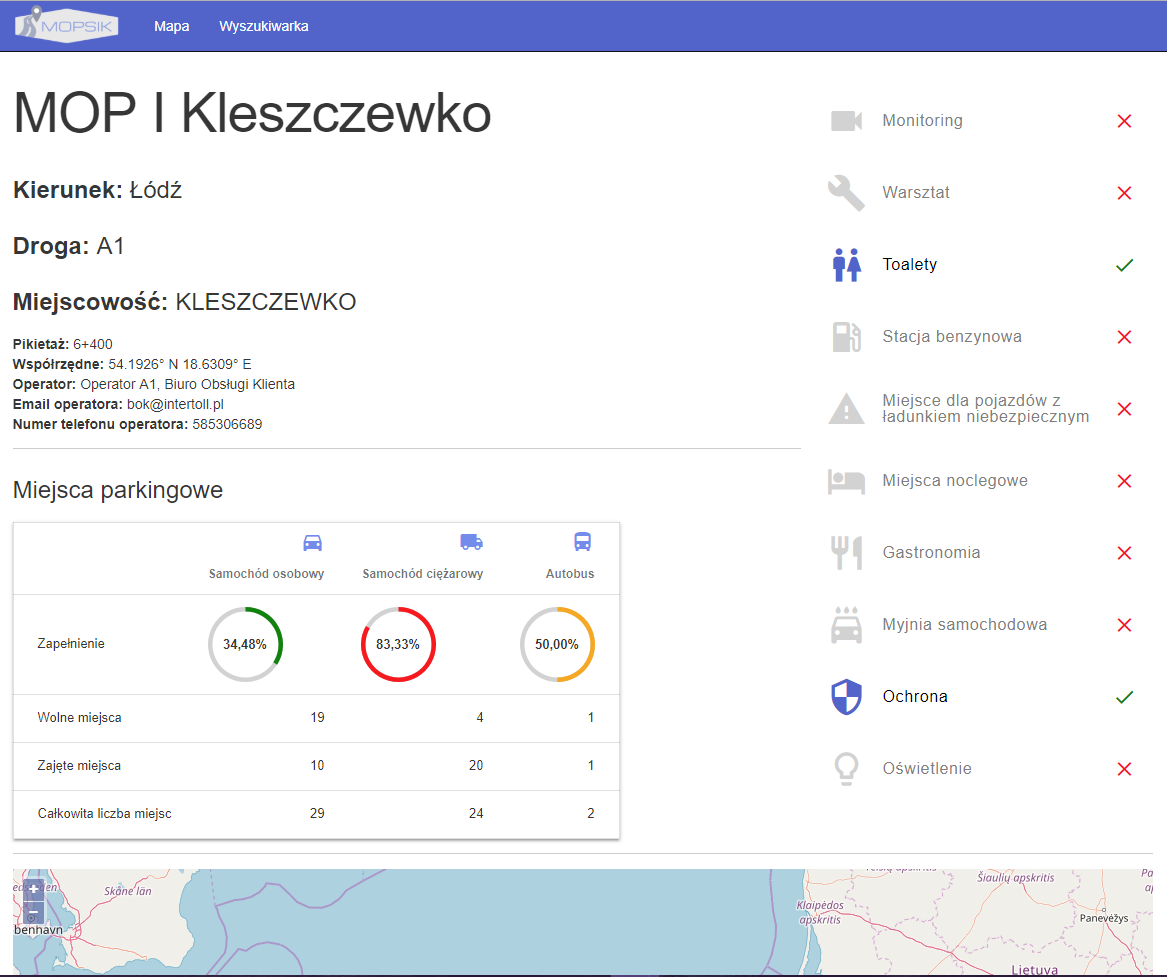
\includegraphics[width=\textwidth]{images/mopsik_www/details1.png}
\captionof{figure}{Szczegóły}
\label{mopsik_www_details}
\end{figure}

\subsection{Zapytania do API i zapisywanie danych}
Aplikacja pobiera wszystkie dane o MOP-ach z opisanego wcześniej API. Wykonuje zapytania do \textit{/mops} i zapisuje je w pamięci aplikacji. Przy każdym przeładowaniu wyświetlanej strony sprawdzane jest jak dawno było wykonane ostatnie zapytanie do API. Jeśli czas ten jest większy niż 2 minuty, zapytanie jest wykonywane ponownie. W przeciwnym przypadku, dane są pobierane z pamięci aplikacji.

\subsubsection{Parsowanie danych z API}
Klasy \textit{Mop}, \textit{Operator}, \textit{FacilitiesParser}, \textit{CoordinatesParser} i \textit{SpacesCount} biorą udział w parsowaniu danych z API, które są w formacie JSON. Przy każdym swoim polu zawierają \textit{JsonProperty} z nazwą pod jaką występują w danych. Dzięki temu, metoda \textit{JsonConvert.DeserializeObject} może sparsować dane w formacie JSON i utworzyć odpowiednie klasy.

\subsection{Modele i modele widoków}
\paragraph{Modele}
\begin{enumerate}
\item \textit{ApiManager} -- odpowiedzialny za zapytania do API, pobiera dane w formacie JSON i zwraca w postaci listy modeli \textit{Mop}
\item \textit{AppDataStorage} -- istnieje jeden obiekt tej klasy, zapisany w aplikacji, można traktować go jako zbiór zmiennych globalnych. Wartości są przechowywane na serwerze, czyli ich wartość jest taka sama dla wszystkich użytkowników. Przechowuje zapisane dane z API oraz czas ostatniego zapytania.
\item \textit{Coordinates} -- dla obu współrzędnych przechowuje ich wartość w formacie \textit{double} oraz w formacie \textit{string} w dwóch wersjach -- zaokrągloną do 4 miejsc po przecinku (do wyświetlania) oraz z pełną dokładnością (do używania w JavaScript). 
\item \textit{CoordinatesParser} -- zawiera obie współrzędne w formacie \textit{double}, używane tylko w parsowaniu danych z API
\item \textit{FacilitiesConfig} -- słownik, który dla kodu symbolizującego usługę na MOP-ie, zwraca obiekt klasy \textit{Facility}
\item \textit{FacilitiesParser} -- zawiera pola \textit{bool} dla każdej usługi, używana tylko w parsowaniu danych z API
\item \textit{Facility} -- zawiera dwie informacje: polską nazwę usługi oraz nazwę ikony
\item \textit{Mop} -- przechowuje wszystkie informacje o MOP-ie; zawiera funkcję \textit{DeserializeMops}, która dla formatu JSON zwraca listę obiektów klasy \textit{Mop}
\item \textit{Operator} -- zawiera pola dla nazwy operatora i kontaktu do niego
\item \textit{SpacesCount} -- zawiera trzy pola \textit{int} (dla każdego z typów pojazdów)
\item \textit{SpacesUsage} -- dla każdego z typów pojazdów zawiera pole klasy \textit{Usage}
\item \textit{Usage} -- zawiera zajętość miejsc parkingowych w \% (w formacie \textit{double} i \textit{string}) oraz odpowiadające tej wartości: kolor tła i tekstu.
\end{enumerate}

\paragraph{Modele widoków}
\begin{enumerate}
\item \textit{DetailsViewModel} -- zawiera \textit{MopViewModel} dla wybranego MOP-a, niezmienny obiekt \textit{FacilitiesConfig} oraz cztery słowniki z odpowiednimi kolorami ikon i tekstu w zależności od obecności usługi
\item \textit{MapViewModel} -- zawiera obiekt klasy \textit{MopListViewModel} z informacjami o wszystkich MOP-ach, aktualny typ pojazdu, dla którego mają być wyświetlane zajętości oraz HTML-owe klasy dla wszystkich trzech przycisków typów pojazdów
\item \textit{MopListViewModel} -- przerabia listę obiektów klasy \textit{Mop} na listę obiektów klasy \textit{MopViewModel}
\item \textit{MopViewModel} -- obudowuje informacje zawarte w klasie \textit{Mop} i przygotowuje je do wyświetlania w widokach
\item \textit{SearchViewModel} -- zawiera m.in informacje o wszystkich MOP-ach, aktualnie wyszukiwane hasło, aktualny stan zaznaczonych ikon w filtrach
\end{enumerate}

\subsection{Kontrolery i widoki}
Dla każdego kontrolera (plik \textit{*Controller.cs}) istnieje plik z HTML (\textit{*.cshtml})
\begin{enumerate}
\item \textit{Details}
\item \textit{Map}
\item \textit{Search}
\end{enumerate}

\subsection{Użyte biblioteki}
\begin{enumerate}
\item \textbf{OpenLayers} \\
\url{https://openlayers.org}\\
Biblioteka napisana w języku JavaScript, umożliwiająca dodawanie dynamicznych map na stronach internetowych.

\item \textbf{Material Design Lite} \\
\url{https://getmdl.io}\\
Biblioteka CSS udostępniająca gotowe style podstawowych elementów HTML. Gwarantuje czysty, spójny wygląd strony internetowej.

\item \textbf{ProgressBar.js} \\
\url{https://github.com/kimmobrunfeldt/progressbar.js}\\
Biblioteka JavaScript do tworzenia animowanych wykresów kołowych. Wykorzystana do rysowania wykresów zajętości MOP-ów.
\end{enumerate}


\chapter{Organizacja pracy}
Nasz projekt składa z się z pięciu częściowo niezależnych programów. Niektóre z nich komunikują lub łączą się ze sobą, ale duża część kodu mogła być napisana bez znajomości szczegółowej implementacji pozostałych aplikacji. Dlatego powstał u nas dość wyraźny podział pracy -- każdy program posiadał swojego koordynatora, który był autorem większości kodu i nadzorował rozwój aplikacji. Dokładny podział prac został przedstawiony w następnym rozdziale. 

\paragraph{Slack}(komunikacja)

Do komunikacji wewnątrz zespołu używaliśmy komunikatora Slack. Daje on możliwość utworzenia wielu kanałów - publicznych i prywatnych, dzięki czemu mogliśmy łatwo rozdzielić rozmowy na poszczególne tematy. Slack umożliwia także przesyłanie plików, do których łatwo dotrzeć w przyszłości. Komunikator można zintegrować z innymi serwisami, np. GitHubem, z którego można dostawać powiadomienia o zmianach w repozytorium.

\paragraph{GitHub}(repozytorium)

Kody źródłowe naszych aplikacji przechowywaliśmy na GitHubie. Utworzyliśmy tam zespół \href{https://github.com/mopsy-team}{\textit{mopsy-team}}, w którym powstało sześć repozytoriów:
\begin{enumerate}
\item Mopnik
\item Mopsim
\item Mopsik-Server
\item Mopsik-Mobile
\item Mopsik-WWW
\item dokumentacja (m.in. praca licencjacka)
\end{enumerate}

\paragraph{Todoist}(menedżer zadań)

Todoist to menadżer zadań, w którym można utworzyć wiele projektów i podprojektów. Wewnątrz każdego z nich można wyznaczać zadania o różnym priorytecie i hierarchii. Każde zadanie można przydzielić jednemu z użytkowników, ustawić termin w jakim ma być wykonane, dodać etykiety i komentować. Aplikacja umożliwia wysyłanie powiadomień o nadchodzących terminach i wykonanych zadaniach.


\chapter{Podział zadań}
\paragraph{Mopnik}
\begin{enumerate}
\item Magdalena Grabowska
\end{enumerate}

\paragraph{Mopsim}
\begin{enumerate}
\item Michał Kukuła
\item Przemysław Perkowski - generowanie planów podróży
\end{enumerate}

\paragraph{Mopsik - serwer}
\begin{enumerate}
\item Przemysław Perkowski
\end{enumerate}

\paragraph{Mopsik - aplikacja mobilna}
\begin{enumerate}
\item Klaudia Laks
\item Przemysław Perkowski - testowanie, code review, poprawki
\end{enumerate}

\paragraph{Mopsik - strona internetowa}
\begin{enumerate}
\item Klaudia Laks
\item Przemysław Perkowski - code review
\end{enumerate}

\paragraph{Dokumentacja / Praca licencjacka}
\begin{enumerate}
\item Magdalena Grabowska
\item Michał Kukuła
\item Klaudia Laks
\item Przemysław Perkowski
\end{enumerate}

\chapter{Napotkane problemy i niezrealizowane pomysły}

Przystępując do zadania, nasza wiedza z zakresu transportu drogowego, w szczególności ciężarowego, była nikła. Podczas realizacji projektu, wdrażając się  w tematykę ruchu na autostradach i drogach szybkiego ruchu, dopiero po pewnym czasie byliśmy w stanie zrozumieć dokładnie jakie funkcjonalności realnie może zapewnić tworzone przez nas oprogramowanie.

W trakcie pisania programów napotkaliśmy wiele problemów oraz wraz z upływem czasu i postępem prac musieliśmy weryfikować, początkowo bardzo ambitny, plan zadań, które uda nam się wykonać.

\section{Napotkane problemy}
Główne problemy, które napotkaliśmy możemy podzielić na kilka podstawowych kategorii:
\begin{enumerate}
\item Problemy z danymi
\item Problemy z komunikacją
\item Problemy techniczne
\end{enumerate}
Po krótce opiszemy każdy z powyższych problemów:
\subsection{Problemy z danymi i komunikacją w zespole}
W ramach projektu RID współpracuje wiele osób, które są odpowiedzialne za różne elementy projektu. 
Dane wymagane do działania naszych programów były pozyskiwane z wielu źródeł, za pośrednictwem wielu osób. Dane te często okazywały się niekompletne lub niewystarczające do naszych zastosowań.
Jednym z przykładów są dane o długości postojów na MOP-ach. Były one zbierane między innymi z:
\begin{itemize}
\item systemu viaTOLL, za pomocą którego były generowane rozkłady czasów przejazdu pomiędzy parą punktów kontroli
\item ankiet przeprowadzanych na MOP-ach. 
\end{itemize}
Okazało się, że otrzymane zbiory danych nie były wystarczające do wiarygodnego wyznaczenia rozkładów czasu podróży. Jedną z czynności, które podjęliśmy w celu uzupełnienia tych danych było stworzenie ankiet internetowych i zamieszczenie ich w portalu Facebook na grupach poświęconych kierowcom samochodów ciężarowych. W związku z niewystarczającymi lub trudnymi do obrobienia danymi, nie zdecydowaliśmy się wprowadzać takiej możliwości.
Innym przykładem są dane o zajętości MOP-ów na żywo. Po początkowych rozmowach z promotorem, jak i~innymi osobami z projektu, wydawało nam się, że do czerwca 2018r. (czyli momentu w którym oddajemy pracę) będą dostępne dane choć z kilku MOP-ów, zapewnione przez zespół z Politechniki Warszawskiej. Po jakimś czasie dowiedzieliśmy się, iż nasze przekonanie jest błędne i dane takie, o ile będą dostępne, to w dalszej przyszłości.
\subsection{Problemy techniczne}
Podczas pracy nad dużym projektem zawsze zdarzają się także problemy techniczne. Nie~inaczej było i tym razem. 
Jednym z przykładów jest praca z React Native, podczas której korzystaliśmy z wielu zewnętrznych bibliotek. Czasem okazywało się, że kolejne wersje tych bibliotek, pobierane z Internetu podczas pracy nad programem zawierały nowe błędy lub luki bezpieczeństwa.

\section{Niezrealizowane pomysły}
Z wyżej wymienionych powodów, nie wszystkie planowane początkowo funkcjonalności udało się wdrożyć do naszych programów.
\subsection{Predycje krótkoterminowe}
Planowaliśmy zaangażować się w analizę danych o zajętości MOP-ów we współpracy z innymi członkami zespołu RID. Na tej podstawie nasza aplikacja mobilna mogłaby nie tylko pokazywać stan zajętości parkingów ,,na żywo'', ale także prognozowaną zajętość za 15, 30, 60 minut. Do analizy tych danych chcieliśmy wykorzystać algorytmy uczenia maszynowego, które dobrze działają przy analizowaniu odcinków czasu, jak np. rekurencyjne sieci neuronowe, czy LSTM. W związku z niewystarczającymi lub trudnymi do obrobienia danymi, nie zdecydowaliśmy się wprowadzać takiej możliwości.
\subsection{Rozszerzona interakcja użytkowników z aplikacją mobilną}
W końcowej fazie tworzenia projektu wpadliśmy na pomysł, jak rozszerzyć aplikację, aby była ona bardziej przydatna dla użytkowników. Można to zrobić w oparciu o crowdsourcing (czyli zaangażowanie dużej grupy ludzi -- użytkowników aplikacji do jakiegoś działania -- dzielenia się informacjami na temat parkingów. Przykładowe funkcjonalności, które sprawiałyby, że użytkownicy pomagaliby sobie wzajemnie byłoby np.
\begin{itemize}
\item ocenianie danego MOP-a poprzez przyznanie mu odpowiedniej liczby gwiazdek
\item podanie jaka konkretnie restauracja znajduje się na danym MOP-ie
\item możliwość dodawania komentarzy do MOP-ów
\end{itemize}
Jeśli pomyślimy o aplikacji w szerszym kontekście, to można byłoby np. dodać też opcję dodawania parkingów niebędących MOP-ami.
Nie zdecydowaliśmy się na wprowadzenie takich usprawnień ze względu na duży czas potrzebny do~dobrego wykonania takiego zadania, biorąc pod uwagę, że do~dopracowania pozostało nam wiele innych funkcjonalności o~większym priorytecie.
\subsection{Precyzyjne dodawanie planowanych dróg do programu Mopnik}
W początkowych fazach projektu planowaliśmy, aby można było nanieść projekt planowanej drogi w~ustalonym formacie na mapę w~Mopniku. Okazało się, że jest to trudne:
\begin{itemize}
\item W początkowych fazach planowania \acrshort{gddkia} nie posiada dokładnych planów dróg.
\item Nasz program musiałby obsługiwać nowy format plików wejściowych, co utrudniłoby implementację.
\end{itemize}
Jako rozwiązanie tego problemu wprowadziliśmy opcję dodawania prostych odcinków pomiędzy punktami A i B na mapie. Ta opcja okazała się o wiele mniej problematyczna w implementacji, a spełnia swój podstawowy cel, tzn. można uruchomić symulację na zmodyfikowanej sieci drogowej i wyznaczyć nowe obiążenia dla odcinków dróg.

\chapter{Zawartość płyty}
%TODO

\begin{thebibliography}{99}
\addcontentsline{toc}{chapter}{Bibliografia}

\bibitem[1]{siec-drogowa-IIIrp} Wikipedia, \textit{Program budowy w III RP},\\ \url{https://pl.wikipedia.org/wiki/Autostrady\_i\_drogi\_ekspresowe\_w\_Polsce}

\bibitem[2]{gddkia-mop} GDDKiA, \textit{Generalna Dyrekcja Dróg Krajowych i Autostrad -- Serwis Informacyjny}, \url{https://www.gddkia.gov.pl/pl/963/miejsca-obslugi-podroznych-mop}

\bibitem[3]{model}Melnik, Roderick. ``Mathematical and Computational Modeling: With Applications in Natural and Social Sciences, Engineering, and the Arts. Wiley.'' ISBN 978-1-118-85398-6., 2015

\bibitem[4]{micmac}Gustafsson, Leif; Sternad, Mikael. ``Bringing consistency to simulation of population models: Poisson Simulation as a bridge between micro and macro simulation''. Mathematical Biosciences. 209: 361–385, 2007

\bibitem[5]{agent-based} Niazi, Muaz; Hussain, Amir. ``Agent-based Computing from Multi-agent Systems to Agent-Based Models: A Visual Survey'', 2011

\bibitem[6]{wiki-agent} Wikipedia, \textit{System wieloagentowy},\\ \url{https://pl.wikipedia.org/wiki/System_wieloagentowy}

\bibitem[7]{matsim} Horni, A, Nagel, K and Axhausen, K W. 2016. ``Introducing MATSim.'' In: Horni, A, Nagel, K and
Axhausen, K W. (eds.) ``The Multi-Agent Transport Simulation MATSim'', Pp. 3–8. London: Ubiquity Press. DOI: http://dx.doi.org/10.5334/baw \\ License: CC-BY 4.0

\bibitem[8]{google-api-faq} Developers Google, \textit{FAQ -- Google Maps API},\\ \url{https://developers.google.com/maps/faq}

\end{thebibliography}

\end{document}


%%% Local Variables:
%%% mode: latex
%%% TeX-master: t
%%% coding: latin-2
%%% End:
